%%%%%%%%%%%%%%%%%%%%%%%%%%%%% Thesis.tex %%%%%%%%%%%%%%%%%%%%%%%%%%%%%%%
%                                                                      %
%  ---------- Master of Science Dissertation template ----------       %
%                                                                      %
%  Template for the Master Thesis according to the regulations         %
%  published by the Academic Board (Direcção Académica) at IST.        %
%                                                                      %
%  For up-to-date guide, please refer to the offical website           %
%  http://da.tecnico.ulisboa.pt/dissertacao-de-mestrado/               %
%                                                                      %
%       Andre C. Marta                                                 %
%       Area Cientifica de Mecanica Aplicada e Aeroespacial            %
%       Departamento de Engenharia Mecanica                            %
%       Instituto Superior Tecnico                                     %
%       Av. Rovisco Pais                                               %
%       1049-001 Lisboa                                                %
%       Portugal                                                       %
%       Tel: +351 21 841 9469                                          %
%                        3469 (extension)                              %
%       Email: andre.marta@tecnico.ulisboa.pt                          %
%                                                                      %
%  Created:       Jan 20, 2011                                         %
%  Last Modified: Jul  2, 2015                                         %
%                                                                      %
%%%%%%%%%%%%%%%%%%%%%%%%%%%%%%%%%%%%%%%%%%%%%%%%%%%%%%%%%%%%%%%%%%%%%%%%
%  Revision history                                                    %
%  v1 - 2011/01/24 - original template                                 %
%  v2 - 2012/10/30 - new IST image and glossary support                %
%  v3 - 2013/12/10 - update according to 2012/13 official guide        %
%  v4 - 2014/02/28 - new default for bibliography style                %
%  v5 - 2014/05/07 - update according to 2013/14 official guide        %
%  v6 - 2015/07/02 - cover page format fixed,                          %
%                    contents page numbering fixed,                    %
%                    better language support,                          %
%                    enhanced examples of tables,                      %
%                    new option for appendix page numbering format,    %
%                    custom bibliography style                         %
%%%%%%%%%%%%%%%%%%%%%%%%%%%%%%%%%%%%%%%%%%%%%%%%%%%%%%%%%%%%%%%%%%%%%%%%
%                                                                      %
% To generate the PDF file, type "make" at the terminal prompt.        %
%                                                                      %
% The IST template LaTeX package was created by the author             %
% and it can be downloaded from:                                       %
% https://fenix.ist.utl.pt/homepage/ist31052/                          %
%                                                                      %
% The external packages can be downloaded from                         %
% the Comprehensive TeX Archive Network at http://www.ctan.org/        %
%                                                                      %
% List of LaTex symbols:                                               %
% http://www.ctan.org/tex-archive/info/symbols/comprehensive/          %
%                                                                      %
% Help with LaTex can be found at                                      %
% http://www.giss.nasa.gov/tools/latex/ltx-2.html                      %
% http://en.wikibooks.org/wiki/LaTeX                                   %
%%%%%%%%%%%%%%%%%%%%%%%%%%%%%%%%%%%%%%%%%%%%%%%%%%%%%%%%%%%%%%%%%%%%%%%%

%%%%%%%%%%%%%%%%%%%%%%%%%%%%%%%%%%%%%%%%%%%%%%%%%%%%%%%%%%%%%%%%%%%%%%%%
%     Preamble                                                         %
%%%%%%%%%%%%%%%%%%%%%%%%%%%%%%%%%%%%%%%%%%%%%%%%%%%%%%%%%%%%%%%%%%%%%%%%

% ----------------------------------------------------------------------
%  Set the document class
% ----------------------------------------------------------------------
\documentclass[10pt,a4paper,twoside]{report}

% ----------------------------------------------------------------------
% Define external packages, language, margins, fonts and new commands
% ----------------------------------------------------------------------
%%%%%%%%%%%%%%%%%%%%%%%%%%%%%%%%%%%%%%%%%%%%%%%%%%%%%%%%%%%%%%%%%%%%%%%%
%                                                                      %
%     File: Thesis_Preamble.tex                                        %
%     Tex Master: Thesis.tex                                           %
%                                                                      %
%     Author: Gonçalo Santos                                           %
%     Last modified : 20 Oct 2018                                      %
%                                                                      %
%%%%%%%%%%%%%%%%%%%%%%%%%%%%%%%%%%%%%%%%%%%%%%%%%%%%%%%%%%%%%%%%%%%%%%%%

% ----------------------------------------------------------------------
% Define document language.
% ----------------------------------------------------------------------

% 'inputenc' package
%
% Accept different input encodings.
% http://www.ctan.org/tex-archive/macros/latex/base/
%
% > allows typing non-english text in LaTeX sources.
%
% ******************************* SELECT *******************************
%\usepackage[latin1]{inputenc} % <<<<< Windows
\usepackage[utf8]{inputenc}   % <<<<< Linux
% ******************************* SELECT *******************************


% 'babel' package
%
% Multilingual support for Plain TeX or LaTeX.
% http://www.ctan.org/tex-archive/macros/latex/required/babel/
%
% > sets the variable names according to the language selected
%
% ******************************* SELECT *******************************
%\usepackage[portuguese]{babel} % <<<<< Portuguese
\usepackage[english]{babel} % <<<<< English
% ******************************* SELECT *******************************


% List of LaTeX variable names: \abstractname, \appendixname, \bibname,
%   \chaptername, \contentsname, \listfigurename, \listtablename, ...
% http://www.tex.ac.uk/cgi-bin/texfaq2html?label=fixnam
%
% Changing the words babel uses (uncomment and redefine as necessary...)
%
\newcommand{\acknowledgments}{@undefined} % new LaTeX variable name
%
% > English
%
\addto\captionsenglish{\renewcommand{\acknowledgments}{Acknowledgments}}
%\addto\captionsenglish{\renewcommand{\listtablename}{List of Tables}}
%\addto\captionsenglish{\renewcommand{\listfigurename}{List of Figures}}
%\addto\captionsenglish{\renewcommand{\nomname}{Nomenclature}}
%\addto\captionsenglish{\renewcommand{\appendixname}{Appendix}}
%\addto\captionsenglish{\renewcommand{\bibname}{References}} % Bibliography

% > Portuguese
%
\addto\captionsportuguese{\renewcommand{\acknowledgments}{Agradecimentos}}
%\addto\captionsportuguese{\renewcommand{\listtablename}{Lista de Figuras}}
%\addto\captionsportuguese{\renewcommand{\listfigurename}{Lista de Tabelas}}
\addto\captionsportuguese{\renewcommand{\nomname}{Lista de S\'{i}mbolos}} % Nomenclatura
%\addto\captionsportuguese{\renewcommand{\appendixname}{Anexo}} % Apendice
%\addto\captionsportuguese{\renewcommand{\bibname}{Refer\^{e}ncias}} % Bibliografia


% ----------------------------------------------------------------------
% Define default and cover page fonts.
% ----------------------------------------------------------------------

% Use Arial font as default
%
\renewcommand{\rmdefault}{phv}
\renewcommand{\sfdefault}{phv}

% Define cover page fonts
%
%         encoding     family       series      shape
%  \usefont{T1}     {phv}=helvetica  {b}=bold    {n}=normal
%                   {ptm}=times      {m}=normal  {sl}=slanted
%                                                {it}=italic
% see more examples at
% http://julien.coron.free.fr/languages/latex/fonts/
%
\def\FontLn{% 16 pt normal
  \usefont{T1}{phv}{m}{n}\fontsize{16pt}{16pt}\selectfont}
\def\FontLb{% 16 pt bold
  \usefont{T1}{phv}{b}{n}\fontsize{16pt}{16pt}\selectfont}
\def\FontMn{% 14 pt normal
  \usefont{T1}{phv}{m}{n}\fontsize{14pt}{14pt}\selectfont}
\def\FontMb{% 14 pt bold
  \usefont{T1}{phv}{b}{n}\fontsize{14pt}{14pt}\selectfont}
\def\FontSn{% 12 pt normal
  \usefont{T1}{phv}{m}{n}\fontsize{12pt}{12pt}\selectfont}


% ----------------------------------------------------------------------
% Define page margins and line spacing.
% ----------------------------------------------------------------------

% 'geometry' package
%
% Flexible and complete interface to document dimensions.
% http://www.ctan.org/tex-archive/macros/latex/contrib/geometry/
%
% > set the page margins (2.5cm minimum in every side, as per IST rules)
%
\usepackage{geometry}	
\geometry{verbose,tmargin=2.5cm,bmargin=2.5cm,lmargin=2.5cm,rmargin=2.5cm}

% 'setspace' package
%
% Set space between lines.
% http://www.ctan.org/tex-archive/macros/latex/contrib/setspace/
%
% > allow setting line spacing (line spacing of 1.5, as per IST rules)
%
\usepackage{setspace}
\renewcommand{\baselinestretch}{1.5}


% ----------------------------------------------------------------------
% Include external packages.
% Note that not all of these packages may be available on all system
% installations. If necessary, include the .sty files locally in
% the <jobname>.tex file directory.
% ----------------------------------------------------------------------

% 'graphicx' package
%
% Enhanced support for graphics.
% http://www.ctan.org/tex-archive/macros/latex/required/graphics/
%
% > extends arguments of the \includegraphics command
%
\usepackage{graphicx}


% 'color' package
%
% Colour control for LaTeX documents.
% http://www.ctan.org/tex-archive/macros/latex/required/graphics/
%
% > defines color macros: \color{<color name>}
%
%\usepackage{color}


% 'amsmath' package
%
% Mathematical enhancements for LaTeX.
% http://www.ctan.org/tex-archive/macros/latex/required/amslatex/
%
% > American Mathematical Society plain Tex macros
%
\usepackage{amsmath}  % AMS mathematical facilities for LaTeX.
\usepackage{amsthm}   % Typesetting theorems (AMS style).
\usepackage{amsfonts} %


% 'wrapfig' package
%
% Produces figures which text can flow around.
% http://www.ctan.org/tex-archive/macros/latex/contrib/wrapfig/
%
% > wrap figures/tables in text (i.e., Di Vinci style)
%
% \usepackage{wrapfig}


% 'subfigure' package
%
% Deprecated: Figures divided into subfigures.
% http://www.ctan.org/tex-archive/obsolete/macros/latex/contrib/subfigure/
%
% > subcaptions for subfigures
%
\usepackage{subfigure}


% 'subfigmat' package
%
% Automates layout when using the subfigure package.
% http://www.ctan.org/tex-archive/macros/latex/contrib/subfigmat/
%
% > matrices of similar subfigures
%
\usepackage{subfigmat}


% 'url' package
%
% Verbatim with URL-sensitive line breaks.
% http://www.ctan.org/tex-archive/macros/latex/contrib/url/
%
% > URLs in BibTex
%
% \usepackage{url}


% 'varioref' package
%
% Intelligent page references.
% http://www.ctan.org/tex-archive/macros/latex/required/tools/
%
% > smart page, figure, table and equation referencing
%
%\usepackage{varioref}


% 'dcolumn' package
%
% Align on the decimal point of numbers in tabular columns.
% http://www.ctan.org/tex-archive/macros/latex/required/tools/
%
% > decimal-aligned tabular math columns
%
\usepackage{dcolumn}
\newcolumntype{d}{D{.}{.}{-1}} % column aligned by the point separator '.'
\newcolumntype{e}{D{E}{E}{-1}} % column aligned by the exponent 'E'


% '' package
%
% Reimplementation of and extensions to LaTeX verbatim.
% http://www.ctan.org/tex-archive/macros/latex/required/tools/
%
% > provides the verbatim environment (\begin{verbatim},\end{verbatim})
%   and a comment environment (\begin{comment},  \end{comment})
%
% \usepackage{verbatim}


% 'moreverb' package
%
% Extended verbatim.
% http://www.ctan.org/tex-archive/macros/latex/contrib/moreverb/
%
% > supports tab expansion and line numbering
%
% \usepackage{moreverb}



% 'nomencl' package
%
% Produce lists of symbols as in nomenclature.
% http://www.ctan.org/tex-archive/macros/latex/contrib/nomencl/
%
% The nomencl package makes use of the MakeIndex program
% in order to produce the nomenclature list.
%
% Nomenclature
% 1: On running the file through LATEX, the command \makenomenclature
%    in the preamble instructs it to create/open the nomenclature file
%    <jobname>.nlo corresponding to the LATEX file <jobname>.tex and
%    writes the information from the \nomenclature commands to this file.
% 2: The next step is to invoke MakeIndex in order to produce the
%    <jobname>.nls file. This can be achieved by making use of the
%    command: makeindex <jobname>.nlo -s nomencl.ist -o <jobname>.nls
% 3: The last step is to invoke LATEX on the <jobname>.tex file once
%    more. There, the \printnomenclature in the document will input the
%    <jobname>.nls file and process it according to the given options.
%
% http://www-h.eng.cam.ac.uk/help/tpl/textprocessing/nomencl.pdf
%
% Nomenclature (produces *.nlo *.nls files)
\usepackage{nomencl}
\makenomenclature
%
% Group variables according to their symbol type
%
\RequirePackage{ifthen}
\ifthenelse{\equal{\languagename}{english}}%
    { % English
    \renewcommand{\nomgroup}[1]{%
      \ifthenelse{\equal{#1}{R}}{%
        \item[\textbf{Roman symbols}]}{%
        \ifthenelse{\equal{#1}{G}}{%
          \item[\textbf{Greek symbols}]}{%
          \ifthenelse{\equal{#1}{S}}{%
            \item[\textbf{Subscripts}]}{%
            \ifthenelse{\equal{#1}{T}}{%
              \item[\textbf{Superscripts}]}{}}}}}%
    }{% Portuguese
    \renewcommand{\nomgroup}[1]{%
      \ifthenelse{\equal{#1}{R}}{%
        \item[\textbf{Simbolos romanos}]}{%
        \ifthenelse{\equal{#1}{G}}{%
          \item[\textbf{Simbolos gregos}]}{%
          \ifthenelse{\equal{#1}{S}}{%
            \item[\textbf{Subscritos}]}{%
            \ifthenelse{\equal{#1}{T}}{%
              \item[\textbf{Sobrescritos}]}{}}}}}%
    }%


% 'glossary' package
%
% Create a glossary.
% http://www.ctan.org/tex-archive/macros/latex/contrib/glossary/
%
% Glossary (produces *.glo *.ist files)
\usepackage[number=none]{glossary}
% (remove blank line between groups)
\setglossary{gloskip={}}
% (redefine glossary style file)
%\renewcommand{\istfilename}{myGlossaryStyle.ist}
\makeglossary


% 'rotating' package
%
% Rotation tools, including rotated full-page floats.
% http://www.ctan.org/tex-archive/macros/latex/contrib/rotating/
%
% > show wide figures and tables in landscape format:
%   use \begin{sidewaystable} and \begin{sidewaysfigure}
%   instead of 'table' and 'figure', respectively.
%
\usepackage{rotating}


% 'hyperref' package
%
% Extensive support for hypertext in LaTeX.
% http://www.ctan.org/tex-archive/macros/latex/contrib/hyperref/
%
% > Extends the functionality of all the LATEX cross-referencing
%   commands (including the table of contents, bibliographies etc) to
%   produce \special commands which a driver can turn into hypertext
%   links; Also provides new commands to allow the user to write adhoc
%   hypertext links, including those to external documents and URLs.
%
\usepackage[pdftex]{hyperref} % enhance documents that are to be
                              % output as HTML and PDF
\hypersetup{colorlinks,       % color text of links and anchors,
                              % eliminates borders around links
%            linkcolor=red,    % color for normal internal links
            linkcolor=black,  % color for normal internal links
            anchorcolor=black,% color for anchor text
%            citecolor=green,  % color for bibliographical citations
            citecolor=black,  % color for bibliographical citations
%            filecolor=magenta,% color for URLs which open local files
            filecolor=black,  % color for URLs which open local files
%            menucolor=red,    % color for Acrobat menu items
            menucolor=black,  % color for Acrobat menu items
%            pagecolor=red,    % color for links to other pages
            pagecolor=black,  % color for links to other pages
%            urlcolor=cyan,    % color for linked URLs
            urlcolor=black,   % color for linked URLs
	          bookmarks=true,         % create PDF bookmarks
	          bookmarksopen=false,    % don't expand bookmarks
	          bookmarksnumbered=true, % number bookmarks
	          pdftitle={Thesis},
            pdfauthor={Andre C. Marta},
            pdfsubject={Thesis Title},
            pdfkeywords={Thesis Keywords},
            pdfstartview=FitV,
            pdfdisplaydoctitle=true}


% 'hypcap' package
%
% Adjusting the anchors of captions.
% http://www.ctan.org/tex-archive/macros/latex/contrib/oberdiek/
%
% > fixes the problem with hyperref, that links to floats points
%   below the caption and not at the beginning of the float.
%
\usepackage[figure,table]{hypcap}


% 'natbib' package
%
% Flexible bibliography support.
% http://www.ctan.org/tex-archive/macros/latex/contrib/natbib/
%
% > produce author-year style citations
%
% \citet  and \citep  for textual and parenthetical citations, respectively
% \citet* and \citep* that print the full author list, and not just the abbreviated one
% \citealt is the same as \citet but without parentheses. Similarly, \citealp is \citep without parentheses
% \citeauthor
% \citeyear
% \citeyearpar
%
\usepackage{natbib}


% ----------------------------------------------------------------------
% Define new commands to assure consistent treatment throughout document
% ----------------------------------------------------------------------

\newcommand{\ud}{\mathrm{d}}                % total derivative
\newcommand{\degree}{\ensuremath{^\circ\,}} % degrees

% Abbreviations

\newcommand{\mcol}{\multicolumn}            % table format

\newcommand{\eqnref}[1]{(\ref{#1})}
\newcommand{\class}[1]{\texttt{#1}}
\newcommand{\package}[1]{\texttt{#1}}
\newcommand{\file}[1]{\texttt{#1}}
\newcommand{\BibTeX}{\textsc{Bib}\TeX}

% Typefaces ( example: {\bf Bold text here} )
%
% > pre-defined
%   \bf % bold face
%   \it % italic
%   \tt % typewriter
%
% > newly defined
\newcommand{\tr}[1]{{\ensuremath{\textrm{#1}}}}   % text roman
\newcommand{\tb}[1]{{\ensuremath{\textbf{#1}}}}   % text bold face
\newcommand{\ti}[1]{{\ensuremath{\textit{#1}}}}   % text italic
\newcommand{\mc}[1]{{\ensuremath{\mathcal{#1}}}}  % math calygraphy
\newcommand{\mco}[1]{{\ensuremath{\mathcalold{#1}}}}% math old calygraphy
\newcommand{\mr}[1]{{\ensuremath{\mathrm{#1}}}}   % math roman
\newcommand{\mb}[1]{{\ensuremath{\mathbf{#1}}}}   % math bold face
\newcommand{\bs}[1]{\ensuremath{\boldsymbol{#1}}} % math symbol
\def\bm#1{\mathchoice                             % math bold
  {\mbox{\boldmath$\displaystyle#1$}}%
  {\mbox{\boldmath$#1$}}%
  {\mbox{\boldmath$\scriptstyle#1$}}%
  {\mbox{\boldmath$\scriptscriptstyle#1$}}}
\newcommand{\boldcal}[1]{{\ensuremath{\boldsymbol{\mathcal{#1}}}}}% math bold calygraphy

\usepackage{fancyvrb}
 % file "Thesis_Preamble.tex"

%%%%%%%%%%%%%%%%%%%%%%%%%%%%%%%%%%%%%%%%%%%%%%%%%%%%%%%%%%%%%%%%%%%%%%%%
%     Begin Document                                                   %
%%%%%%%%%%%%%%%%%%%%%%%%%%%%%%%%%%%%%%%%%%%%%%%%%%%%%%%%%%%%%%%%%%%%%%%%
\begin{document}

% Set plain page style (no headers, footer with centered page number)
\pagestyle{plain}

% Set roman numbering (i,ii,...) before the start of chapters
\pagenumbering{roman}

% ----------------------------------------------------------------------
%  Cover page
% ----------------------------------------------------------------------
%%%%%%%%%%%%%%%%%%%%%%%%%%%%%%%%%%%%%%%%%%%%%%%%%%%%%%%%%%%%%%%%%%%%%%%%
%                                                                      %
%     File: Thesis_FrontCover.tex                                      %
%     Tex Master: Thesis.tex                                           %
%                                                                      %
%     Author: Gonçalo Santos                                           %
%     Last modified : 20 Oct 2018                                      %
%                                                                      %
%%%%%%%%%%%%%%%%%%%%%%%%%%%%%%%%%%%%%%%%%%%%%%%%%%%%%%%%%%%%%%%%%%%%%%%%

\thispagestyle {empty}

% IST Logo
% parameters: bb=llx lly urx ury (bounding box), width=h_length, height=v_length, angle=angle, scale=factor, clip=true/false, draft=true/false.
\vspace*{-12mm}
\hspace*{-12mm}

\includegraphics[height=20mm]{IST_A_CMYK_POS-crop.pdf}

\begin{center}
%
% Figure (Image or plot)
\vspace{0.5cm}
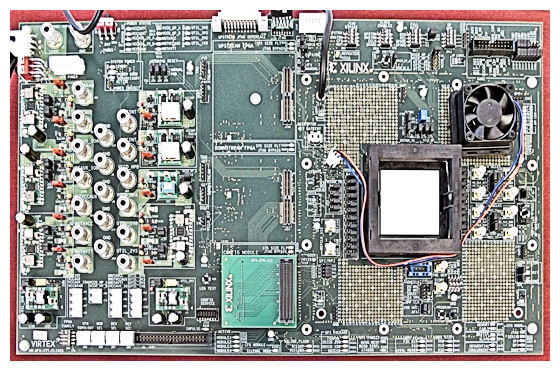
\includegraphics[height=60mm]{Figures/fpga.jpg}

% Title, author and degree
\vspace{0.8cm}
{\FontLb C Compiler for the VERSAT Reconfigurable Processor} \\
\vspace{3.6cm}
{\FontMb Gonçalo da Conceição Reis dos Santos} \\
\vspace{1.9cm}
{\FontLn Thesis to obtain the Master of Science Degree in} \\
\vspace{0.3cm}
{\FontLb Electrical and Computer Engineering} \\
%\vspace{1.9cm}
\vspace{1.0cm}
{\FontSn %
\begin{tabular}{ll}
Supervisor: & Prof. José João Henriques Teixeira de Sousa
\end{tabular} } \\
\vspace{1.0cm}
{\FontMb Examination Committee} \\
\vspace{0.3cm}
{\FontSn %
\begin{tabular}{ll}
Chairperson: & Prof. Francisco André Corrêa Alegria\\
Supervisor: & Prof. José João Henriques Teixeira de Sousa \\
Member of the Committee: & Prof. Paulo Ferreira Godinho Flores \\
\end{tabular} } \\
\vspace{1.5cm}
{\FontMb November 2019} \\
%
\end{center}

\cleardoublepage
 % file "Thesis_FrontCover.tex"
\cleardoublepage

% ----------------------------------------------------------------------
% Dedication page (optional)
% ----------------------------------------------------------------------
%%%%%%%%%%%%%%%%%%%%%%%%%%%%%%%%%%%%%%%%%%%%%%%%%%%%%%%%%%%%%%%%%%%%%%%%%
%                                                                      %
%     File: Thesis_Dedication.tex                                      %
%     Tex Master: Thesis.tex                                           %
%                                                                      %
%     Author: Andre C. Marta                                           %
%     Last modified :  2 Jul 2015                                      %
%                                                                      %
%%%%%%%%%%%%%%%%%%%%%%%%%%%%%%%%%%%%%%%%%%%%%%%%%%%%%%%%%%%%%%%%%%%%%%%%

\null\vskip5cm%
\begin{flushright}
     Dedicated to someone special...
\end{flushright}
\vfill\newpage

 % file "Thesis_Dedication.tex"
%\cleardoublepage

% ----------------------------------------------------------------------
%  Acknowledgments (optional)
% ----------------------------------------------------------------------
%%%%%%%%%%%%%%%%%%%%%%%%%%%%%%%%%%%%%%%%%%%%%%%%%%%%%%%%%%%%%%%%%%%%%%%%%
%                                                                      %
%     File: Thesis_Acknowledgments.tex                                 %
%     Tex Master: Thesis.tex                                           %
%                                                                      %
%     Author: Andre C. Marta                                           %
%     Last modified :  2 Jul 2015                                      %
%                                                                      %
%%%%%%%%%%%%%%%%%%%%%%%%%%%%%%%%%%%%%%%%%%%%%%%%%%%%%%%%%%%%%%%%%%%%%%%%

\section*{\acknowledgments}

% Add entry in the table of contents as section
\addcontentsline{toc}{section}{\acknowledgments}

I want to thank my supervisor, Professor José Teixeira de Sousa, for the 
opportunity to develop this work and for his guidance and support during that process. 
His help was fundamental to overcome the multiple obstacles that I faced during this work.

I also want to acknowledge Professor Horácio Neto for providing a simple Convolutional 
Neural Network application, used as a basis for the application developed for the 
RV32-Versat architecture.

A special acknowledgement goes to my friends, for their continuous support, and Válter,  
that is developing a multi-layer architecture for RV32-Versat. When everything seemed to 
be doomed he always had a miraculous solution.

Finally, I want to express my sincere gratitude to my family for giving me all the 
support and encouragement that I needed throughout my years of study and through the 
process of researching and writing this thesis. They are also part of this work.\\

\textbf{Thank you.}

 % file "Thesis_Acknowledgements.tex"
%\cleardoublepage

% ----------------------------------------------------------------------
%  Abstract (both in English and Portuguese)
% ----------------------------------------------------------------------
%%%%%%%%%%%%%%%%%%%%%%%%%%%%%%%%%%%%%%%%%%%%%%%%%%%%%%%%%%%%%%%%%%%%%%%%
%                                                                      %
%     File: Thesis_Abstract.tex                                        %
%     Tex Master: Thesis.tex                                           %
%                                                                      %
%     Author: Andre C. Marta                                           %
%     Last modified :  2 Jul 2015                                      %
%                                                                      %
%%%%%%%%%%%%%%%%%%%%%%%%%%%%%%%%%%%%%%%%%%%%%%%%%%%%%%%%%%%%%%%%%%%%%%%%

\section*{Abstract}

% Add entry in the table of contents as section
\addcontentsline{toc}{section}{Abstract}

Versat is a Coarse-Grain Reconfigurable Array architecture (CGRA), which
implements self and partial reconfiguration by using a simple controller
unit. This report studies the current state of the art in HDL and CGRA
simulation, providing a basis to the development of a simulation environment for
Versat. The main objective of this environment is to provide a faster way to
develop and debug software without the use of prototyping hardware. Therefore,
the two types of HDL simulators, event-driven and cycle-accurate, their
advantages and disadvantages are studied, along with a performance comparison
between them. A study of high-level implementations for CGRA simulation is
also presented.

\vfill

\textbf{\Large Keywords:} Versat, coarse-grain reconfigurable arrays, HDL
simulation, CGRA simulation, high-level simulation

 % file "Thesis_Abstract.tex"
\cleardoublepage

%%%%%%%%%%%%%%%%%%%%%%%%%%%%%%%%%%%%%%%%%%%%%%%%%%%%%%%%%%%%%%%%%%%%%%%%
%                                                                      %
%     File: Thesis_Resumo.tex                                          %
%     Tex Master: Thesis.tex                                           %
%                                                                      %
%     Author: Carlos A. Rodrigues                                           %
%     Last modified : 21 Jan 2011                                      %
%                                                                      %
%%%%%%%%%%%%%%%%%%%%%%%%%%%%%%%%%%%%%%%%%%%%%%%%%%%%%%%%%%%%%%%%%%%%%%%%

\section*{Resumo}

% Add entry in the table of contents as section
\addcontentsline{toc}{section}{Resumo}

Inserir o resumo em Portugu\^{e}s aqui com o máximo de 250 palavras e acompanhado de 4 a 6 palavras-chave...

\vfill

\textbf{\Large Palavras-chave:} OpenRISC, Sistema em um chip,...

\cleardoublepage

   % file "Thesis_Resumo.tex"
\cleardoublepage

% ----------------------------------------------------------------------
%  Table of contents, list of tables, list of figures and nomenclature
% ----------------------------------------------------------------------

%\glsunsetall

% Table of contents
%
\tableofcontents
\cleardoublepage 

% List of tables
%
% Add entry in the table of contents as section
\phantomsection
\addcontentsline{toc}{section}{\listtablename}
% Generate list
\listoftables
\cleardoublepage 

% List of figures
%
% Add entry in the table of contents as section
\phantomsection
\addcontentsline{toc}{section}{\listfigurename}
% Generate list
\listoffigures
\cleardoublepage 

% Nomenclature
%
% entries of nomenclature list
%%%%%%%%%%%%%%%%%%%%%%%%%%%%%%%%%%%%%%%%%%%%%%%%%%%%%%%%%%%%%%%%%%%%%%%%%
%                                                                      %
%     File: Thesis_Nomenclature.tex                                    %
%     Tex Master: Thesis.tex                                           %
%                                                                      %
%     Author: Gonçalo Santos                                           %
%     Last modified : 20 Oct 2018                                      %
%                                                                      %
%%%%%%%%%%%%%%%%%%%%%%%%%%%%%%%%%%%%%%%%%%%%%%%%%%%%%%%%%%%%%%%%%%%%%%%%
%
% The definitions can be placed anywhere in the document body
% and their order is sorted by <symbol> automatically when
% calling makeindex in the makefile
%
% The \glossary command has the following syntax:
%
% \glossary{entry}
%
% The \nomenclature command has the following syntax:
%
% \nomenclature[<prefix>]{<symbol>}{<description>}
%
% where <prefix> is used for fine tuning the sort order,
% <symbol> is the symbol to be described, and <description> is
% the actual description.

% ----------------------------------------------------------------------
% Roman symbols [r]
\nomenclature[ru]{$\bf u$}{Velocity vector.}
\nomenclature[ru]{$u,v,w$}{Velocity Cartesian components.}
\nomenclature[rp]{$p$}{Pressure.}
\nomenclature[rC]{$C_D$}{Coefficient of drag.}
\nomenclature[rC]{$C_L$}{Coefficient of lift.}
\nomenclature[rC]{$C_M$}{Coefficient of moment.}

% ----------------------------------------------------------------------
% Greek symbols [g]
\nomenclature[g]{$\rho$}{Density.}
\nomenclature[g]{$\alpha$}{Angle of attack.}
\nomenclature[g]{$\beta$}{Angle of side-slip.}
\nomenclature[g]{$\mu$}{Molecular viscosity coefficient.}
\nomenclature[g]{$\kappa$}{Thermal conductivity coefficient.}

% ----------------------------------------------------------------------
% Subscripts [s]
\nomenclature[s]{$x,y,z$}{Cartesian components.}
\nomenclature[s]{$i,j,k$}{Computational indexes.}
\nomenclature[s]{$\infty$}{Free-stream condition.}
\nomenclature[s]{ref}{Reference condition.}
\nomenclature[s]{$n$}{Normal component.}

% ----------------------------------------------------------------------
% Supercripts [t]
\nomenclature[t]{T}{Transpose.}
\nomenclature[t]{*}{Adjoint.}

 % file "Thesis_Nomenclature.tex"
%
% Add entry in the table of contents as section
%\phantomsection
%\addcontentsline{toc}{section}{\nomname}
% Insert glossary/nomenclature section produced by MakeIndex
%\printnomenclature
%\cleardoublepage

% entries of glossary list
%%%%%%%%%%%%%%%%%%%%%%%%%%%%%%%%%%%%%%%%%%%%%%%%%%%%%%%%%%%%%%%%%%%%%%%%%
%                                                                      %
%     File: Thesis_Glossary.tex                                        %
%     Tex Master: Thesis.tex                                           %
%                                                                      %
%     Author: Carlos A. Rodrigues                                           %
%     Last modified : 30 Oct 2012                                      %
%                                                                      %
%%%%%%%%%%%%%%%%%%%%%%%%%%%%%%%%%%%%%%%%%%%%%%%%%%%%%%%%%%%%%%%%%%%%%%%%
%
% The definitions can be placed anywhere in the document body
% and their order is sorted by <symbol> automatically when
% calling makeindex in the makefile
%
% The \glossary command has the following syntax:
%
% \glossary{entry}
%
% The \nomenclature command has the following syntax:
%
% \nomenclature[<prefix>]{<symbol>}{<description>}
%
% where <prefix> is used for fine tuning the sort order,
% <symbol> is the symbol to be described, and <description> is
% the actual description.

% ----------------------------------------------------------------------

\glossary{name={\textbf{MDO}},description={Multi-Disciplinar Optimization is an engineering technique that uses optimization methods to solve design problems incorporating two or more disciplines.}}

\glossary{name={\textbf{CFD}},description={Computational Fluid Dynamics is a branch of fluid mechanics that uses numerical methods and algorithms to solve problems that involve fluid flows.}}

\glossary{name={\textbf{CSM}},description={Computational Structural Mechanics is a branch of structure mechanics that uses numerical methods and algorithms to perform the analysis of structures and its components.}}

 % file "Thesis_Glossary.tex"

% Add entry in the table of contents as section
%\phantomsection
%\addcontentsline{toc}{section}{\glossaryname}
% Insert glossary section produced by MakeIndex
%\printglossary[type=\acronymtype]
%\printglossaries
%\printacronyms

\phantomsection
\chapter*{List of Acronyms}
% Add entry in the table of contents as section
\addcontentsline{toc}{section}{List of Acronyms}
%\begin{acronym}[CGRA]
\newacro{CGRA}{Coarse-Grain Reconfigurable Array}
\newacro{CPU}{Central Processing Unit}
\newacro{ISA}{Instruction Set Architecture}
\newacro{UART}{Universal Asynchronous Receiver-Transmitter}
\newacro{LED}{Light Emitting Diode}
\newacro{CM}{Configuration Module}
\newacro{DE}{Data Engine}
\newacro{FU}{Functional Units}
\newacro{AGU}{Address Generation Unit}
\newacro{LUT}{Lookup Tables}
\newacro{FPGA}{Field-Programmable Gate Array}
\newacro{ASIC}{Application-Specific Integrated Circuit}
\newacro{CPI}{Cycles Per Instruction}
\newacro{CNN}{Convolutional Neural Network}
\newacro{HDL}{Hardware Description Language}
\newacro{RTL}{Register-Transfer Level}
\newacro{UUT}{Unit Under Test}
\newacro{VPI}{Verilog Procedural Interface}
\newacro{API}{Application Programming Interface}
\newacro{DMA}{Direct Memory Access}
\newacro{VCD}{Value Change Dump}
\newacro{BRAM}{Block Random Access Memories}
\newacro{DSP}{Digital Signal Processor}
\newacro{ASIP}{Application Specific Instruction Set Processors}
\newacro{ALU}{Arithmetic Logic Unit}
%\end{acronym}
%print list

\noindent
\textbf{AGU} Address Generation Unit\\
\textbf{ALU} Arithmetic Logic Unit\\
\textbf{API} Application Programming Interface\\
\textbf{ASIC} Application-Specific Integrated Circuit\\
\textbf{ASIP} Application Specific Instruction Set Processor\\
\textbf{BRAM} Block Random Access Memory\\
\textbf{CGRA} Coarse-Grain Reconfigurable Array\\
\textbf{CM} Configuration Module\\
\textbf{CNN} Convolutional Neural Network\\
\textbf{CPI} Cycles Per Instruction\\
\textbf{CPU} Central Processing Unit\\
\textbf{DE} Data Engine\\
\textbf{DMA} Direct Memory Access\\
\textbf{DSP} Digital Signal Processor\\
\textbf{FPGA} Field-Programmable Gate Array\\
\textbf{FU} Functional Unit\\
\textbf{HDL} Hardware Description Language\\
\textbf{ISA} Instruction Set Architecture\\
\textbf{LED} Light Emitting Diode\\
\textbf{LUT} Lookup Table\\
\textbf{RTL} Register-Transfer Level\\
\textbf{UART} Universal Asynchronous Receiver-Transmitter\\
\textbf{UUT} Unit Under Test\\
\textbf{VCD} Value Change Dump\\
\textbf{VPI} Verilog Procedural Interface\\ % file "Thesis_Acronyms.tex"
\cleardoublepage

% Set arabic numbering (1,2,...) after preface
%
\setcounter{page}{1}
\pagenumbering{arabic}

% ----------------------------------------------------------------------
%  Chapters
% ----------------------------------------------------------------------

%\glsresetall

%%%%%%%%%%%%%%%%%%%%%%%%%%%%%%%%%%%%%%%%%%%%%%%%%%%%%%%%%%%%%%%%%%%%%%%%
%                                                                      %
%     File: Thesis_Introduction.tex                                    %
%     Tex Master: Thesis.tex                                           %
%                                                                      %
%     Author: Andre C. Marta                                           %
%     Last modified :  2 Jul 2015                                      %
%                                                                      %
%%%%%%%%%%%%%%%%%%%%%%%%%%%%%%%%%%%%%%%%%%%%%%%%%%%%%%%%%%%%%%%%%%%%%%%%

\chapter{Introduction}
\label{chapter:introduction}




In this report, the problem of accelerating the execution of Deep Neural
Networks (DNNs) using Coarse GRained Reconfigurable Arrays (CGRAs) is studied,
with special emphasis on compiling a DNN description into code that runs on
CPU/CGRA system. The Deep Versat Architecture~\cite{valter:deepversat} CGRA will be used as an
implementation tool in this work.


%%%%%%%%%%%%%%%%%%%%%%%%%%%%%%%%%%%%%%%%%%%%%%%%%%%%%%%%%%%%%%%%%%%%%%%%
\section{Problem}
\label{section:problem}

Neural Networks have been an object of study since the 1940's, but until the
beginning of this decade their applications were limited and did not play a
major role in computer vision conferences. With its meteoric rise in research,
several solutions to accelerate this algorithm have appeared, from Field Programmable Gate Arrays (FPGA) to
Application Specific Integrated Circuits (ASIC) implementations.

Convolutional Neural Networks (CNNs) are a particular kind of DNN where the output
values of the neurons in one layer are convolved with a kernel to produce the
input values of the neurons of the next layer. This algorithm is compute bound,
that is, its performance depends on how fast it can do certain calculations, and
depend less on the memory access time. Namely the convolutional layers take
approximately 90$\%$ of the computation time.

The acceleration of these workloads is a matter of importance for today's
applications such as image processing for object recognition or simply to
enhance certain images. Other uses like instant translation and virtual
assistants are applications of neural networks and their acceleration is of
vital importance to bring them into Internet of Things.

A suitable circuit to accelerate DNNs in hardware is the CGRA. A CGRA is a
collection of Functional Units and memories with programmable interconnections
in order to form computational datapaths. A CGRA can be implemented in both
FPGAs and ASICs. CGRAs can be reconfigured much faster than FPGAs, as they have
much less configuration bits. If reconfiguration is done at runtime, CGRAs add
temporal scalability to the spacial scalability that characterize
FPGAs. Moreover, partial reconfiguration is much easier to do in CGRAs compared
to FPGAs which further speeds up reconfiguration time. Another advantage of
CGRAs is the fact that they can be programmed entirely in software, contrasting
with the large development time of customized Intellectual Property (IP) blocks.
The Coarse Grain Reconfigurable Arrays (CGRA) is a midway acceleration solution
between FPGAs, which are flexible but large, power hungry and difficult to
reprogram, and ASICs, which are fast but generally not programmable.

However, mapping a specific DNN to a CGRA requires knowledge of its
architecture, latencies and register configurations, which may become a lengthy
process, especially if the user wants to explore the design space for several
DNN configurations. An automatic compiler that can map a standard DNN
description into CPU/CGRA code would dramatically decrease time to market of its
users. Currently there are equivalent tools for CPUs and GPUs and
even for FPGAS.


%%%%%%%%%%%%%%%%%%%%%%%%%%%%%%%%%%%%%%%%%%%%%%%%%%%%%%%%%%%%%%%%%%%%%%%%
\section{Solution}
\label{section:solution}

The proposed solution is a compiler that takes a configuration file from a
neural network framework like Caffe or Darknet. This new tool inputs the
parameters of Deep Versat, such as the number of layers and functional units,
and produces the C code needed for the Versat runs. This code is run on the
RISC-V picorv32~\cite{picorv} CPU controller that has Deep Versat as a peripheral.

%%%%%%%%%%%%%%%%%%%%%%%%%%%%%%%%%%%%%%%%%%%%%%%%%%%%%%%%%%%%%%%%%%%%%%%%
%\section{Thesis Outline}
%\label{section:outline}

%Briefly explain the contents of the different chapters...

%%%%%%%%%%%%%%%%%%%%%%%%%%%%%%%%%%%%%%%%%%%%%%%%%
%\section{Author's Work}
%\label{section:authorwork}

%TO ADD----

%%%%%%%%%%%%%%%%%%%%%%%%%%%%%%%%%%%%%%%%%%%%%%%%%%
\section{Report Outline}
\label{reportoutline}

This report is composed of 4 more chapters. In the second chapter, the
state-of-the-art of neural networks and the difficulties accelerating them is
described. In the third chapter, the Deep Versat architecture and how to program
it is explained. In the fourth chapter, CNN compiler techniques are
explored. Finally, the last chapter contains the proposed solution and the plan
for its execution.


 % file "Thesis_Introduction.tex"
\cleardoublepage

\chapter{CNN Background}
\label{chapter:background}

%This chapter is the main one for the IIEEC report, it contains the section about \textbf{Framing of the thesis theme in the scientific area and state of the art revision}.
%%%%%%%%%%%%%%%%%%%%%%%%%%%%%%%%%%%%%%%%%%%%%%%%%%%%%%%%%%%%%%%%%%%%%%%%%
%
%Things I need to talk about:
%\begin{itemize}
%    \item What are neural networks being used for - general introduction
%    \item architecture of neural networks: more terminology: input, output, hidden layers...
%    \item Training vs Inference
%    \item Basic neural network operations: weights, biases, Activations (Fully Connected Layer)
%    \item Deep neural networks: advantages, difficulties
%    \item Convolutional Neural Networks (CNN): basic operation, some intuition, results (e.g ImageNet)
%    \item 3 basic ideias of CNNs: local receptive fields, shared weights, pooling
%    \item introduce terminology: kernel/filter, feature map
%    \item putting all factors that make DNNs, more specifically CNNs work
%    \item factors for effective training (and problems)
%\end{itemize}{}
%
%\newpage

Convolutional neural networks (CNNs) were introduced in 1989 by Yann LeCun for
digit recognition~\cite{lecun:handwritten_zipcodes89}. Since then CNNs have
increased in size and complexity and have gained popularity in the last years
for applications like speech processing, robotics and image processing. One
example is the performance of AlexNet~\cite{AlexNetKrizhevsky:2012} at the
ImageNet Large Scale Visual Recognition Challenge
2012~\cite{ImageNet2012_ILSVRC15}.

In this chapter a background for CNNs is established. The first sections
introduce the concepts of inference and training of neural networks. Then, the
main types of layers found in CNNs are presented. In the final part of the
chapter, an analysis of the YOLOv3~\cite{yolov3} network, a CNN used for image
detection, is presented.


%Since the result of the AlexNet \cite{AlexNetKrizhevsky:2012} at the ImageNet Large Scale Visual Recognition Challenge 2012 \cite{ImageNet2012_ILSVRC15}, convolutional neural networks have been used for image recognition applications.

\section{Neural Networks}
\label{section:neural_networks}

% Neural networks have gained popularity in the last years due to accuracy on applications like speech processing, robotics and image processing.
\begin{figure}[!htb]
	\centering
	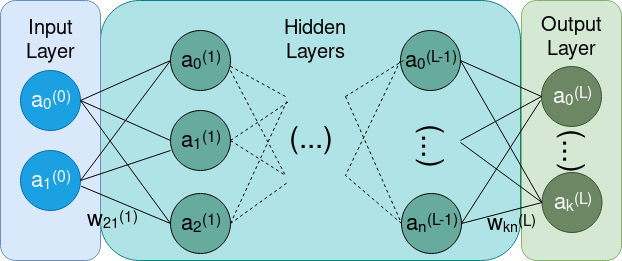
\includegraphics[width=0.70\textwidth]{Figures/FCNN.png}
	\caption[Caption for figure in TOC.]{Neural Network Structure}
	\label{fig:FCNN}
\end{figure}

The most basic element of neural networks is the neuron. The output value $a$ of
a neuron is given by
\begin{equation}
a  = \sigma\Big( b + \sum_{i=0}^{n-1} w_{i}\times x_i \Big),
\label{eq:neuron_value}
\end{equation}
where $w_i$ is the weight associated with input $x_i$, $b$ is a parameter called
bias, $\sigma(.)$ is called the activation function and $n$ is the number of
inputs of the neuron.

Fig.~\ref{fig:FCNN} presents a neural network. Neurons are organized in layers
where the neurons in one layer only receive input values from the same set of
previous layers. If the input values are the neural network inputs, the layer is
called the \underline{input layer}. The values calculated at the input layer
neurons are sent to the next layer. The last layer of the network is called the
\underline{output layer}. The layers in between are called \underline{hidden
  layers}.

Activations are non-linear functions applied to each neuron output. The non-linearity
of the activation functions allows for multiple layer networks to approximate
any function~\cite{mnielsen:nnanddl}. The sigmoid function, presented in
Fig.~\ref{fig:sigmoid}, is one of the first functions used. In the last years,
the Rectified Linear Unit (ReLU), Fig.~\ref{fig:ReLU}, and some variations like
the leaky ReLU, Fig.~\ref{fig:leaky}, have gained popularity due to the reduced
computational complexity during network training.
%\begin{equation}
%\begin{cases}
%Sigmoid(x) = \frac{1}{1 + \exp(-x)} \\
%ReLU(x) = max\{0, x \}\\
%Leaky_{ReLU}(x) = max\{0.1x, x\}
%\label{eq:activation_functions}
%\end{cases}
%\end{equation}

\begin{figure}[!htb]
	\begin{subfigmatrix}{3}
		\subfigure[Sigmoid Activation]{\label{fig:sigmoid} 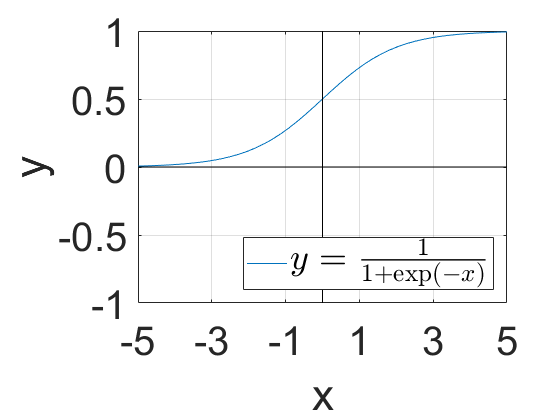
\includegraphics[width=0.32\textwidth]{Figures/sigmoid.png}}
		\subfigure[ReLU Activation]{\label{fig:ReLU} 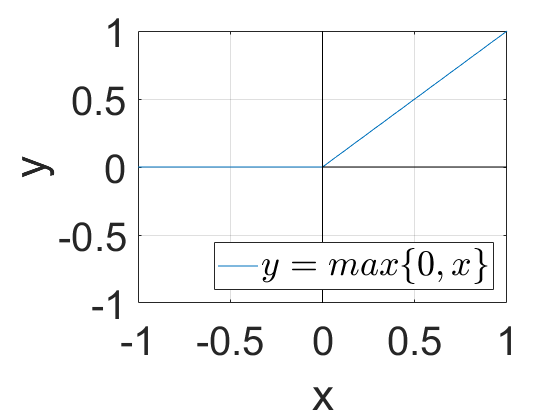
\includegraphics[width=0.32\textwidth]{Figures/ReLU.png}}
		\subfigure[Leaky ReLU Activation]{\label{fig:leaky} 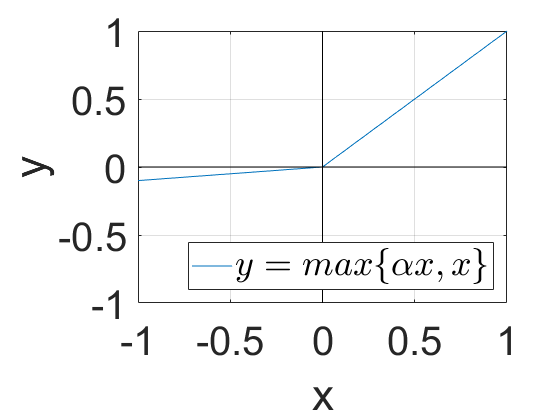
\includegraphics[width=0.32\textwidth]{Figures/leaky_ReLU.png}}		
	\end{subfigmatrix}
	\caption{Plots of common activation functions}
	\label{fig:activation_plots}
\end{figure}

\section{Neural Network Inference}
\label{section:inference}
Inference corresponds to the operation of the network over data outside of the
training dataset using the already trained weights and biases. The key idea
behind this mode is that if the input data being received is similar to the data
used for training, then the output generated by the network should reach a
comparable accuracy with the one achieved during training.

\section{Neural Network Training}
\label{section:training}
Neural networks are trained using a training dataset that contains inputs for
the network and the desired outputs. During training, the weights and biases of
the network are tuned so that given the dataset inputs, the output generated is
as close as possible to the desired output. Training is based on gradient
descent techniques that update the weights and biases of the network based on
the partial derivatives of each value with respect to the difference between the
desired output and the one generated by the network. The backpropagation
algorithm is the main method used for network training. Training is demanding in
terms of computation and memory. The training process is often done in a
separate machine, usually taking advantage of the computation capabilities of
GPUs.

\section{Fully-Connected Network}
\label{subsection:fc_network}

In fully-connected layers, each neuron receives the outputs from all neurons of
the previous layer, where there is a different weight associated for each input
value. In fact, Fig.~\ref{fig:FCNN} depicts a neural network composed
exclusively by fully-connected layers.


%In general the fully-connected layers appear at the end of the network to perform the classification of the features detected by the convolutional layers.

%intro to deep neural networks into CNNs
% 3 basic ideias - introduce terminology
% talk about convolution - pooling - normalization - activations
% quantitative factors to CNNs (throughout the previous text?)

%\subsection{Deep Neural Networks (DNNs)}
%\label{subsection:dnns}
%For the application of image processing, the intuition of how the network works is related with each neuron being able to detect one pattern. With more layers, the neurons on the first layers detect simple patterns that are progressively compounded into more complex patterns across the layers, up to the output layer, where the object detection is done. Following this logic, it is expected that deep neural networks can be more powerful than a shallow network. However, this comes with additional difficulties in training all the weights and biases for networks of increasing depth. This problem is usually circumvented by replacing the fullyconnected layers with convolutional layers.

\section{Convolutional Neural Networks (CNNs)}
\label{section:cnns}

Unlike fully-connected networks, CNNs are mainly composed by convolutional
layers. Other commonly found layers in CNNs are pooling, batch normalization,
routing, upsample and shortcut layers.

% Convolutional neural networks are based on three basic ideas: \underline{local receptive fields}, \underline{shared weights} and \underline{pooling} \cite{mnielsen:nnanddl}.


\subsection{Convolutional Layer}
\label{subsection:conv_layer}

In convolutional layers, a neuron only depends on a small number of inputs,
which corresponds to the neuron only analysing a specific feature for a region
of the input. The specific region is called local receptive
  field. Hence, associated with each neuron, there is only a reduced number of
weights and one bias.

In fact, the same local weights and bias are used for a set of neurons, which
corresponds to searching for the same feature in the entire input, making
convolution invariable to translation in images. The shared weights form a
\underline{kernel}.

%This process creates a \underline{feature map (FM)} of the input, due to using the same \underline{shared weights} and \underline{shared bias} over a small region that is overlapped onto an image like a sliding window. 
% and for each layer multiple kernels can be used to generate multiple corresponding feature maps.

The input of convolutional layers is divided into $C$ channels, where each
channel is defined as a ($W\times H$) \underline{feature map (FM)}. For example,
in Fig.~\ref{fig:3D_conv} the input has 3 channels and each feature map has size
$6\times 6$.

Each kernel used in the convolution has $C$ channels, the same as the input. The
number of output channels is the same as the number of kernels used. Each value
on the output is the accumulation of the products of the input with the
overlapped kernel.

\begin{figure}[!htb]
	\centering
	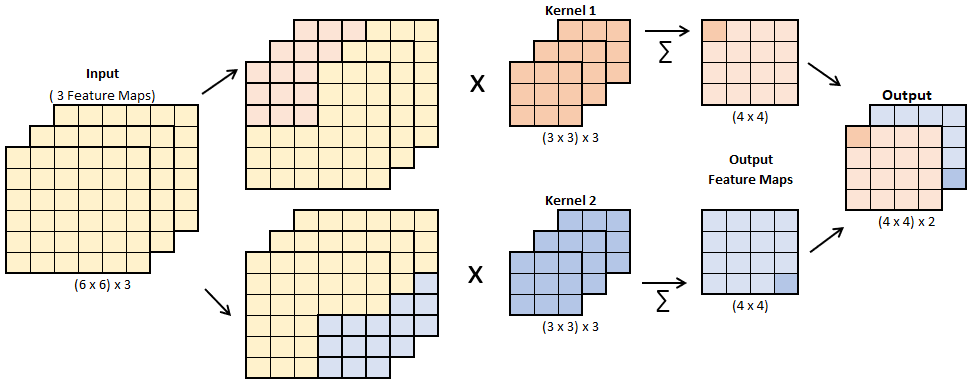
\includegraphics[width=0.70\textwidth]{Figures/3D_convolution.png}
	\caption[Caption for figure in TOC.]{Example of a 3D convolution}
	\label{fig:3D_conv}
\end{figure}

%Fig. \ref{fig:3D_conv} presents an example of a 3D convolution. Given an input composed of multiple feature maps (channels), multiple three dimensional kernels with the same number of channels are used for convolution, creating one output feature map per kernel. The number of output channels is the same as the number of kernels used. Each value on the output is the accumulation of the products of the input with the overlapped kernel.

\subsection{Pooling Layer}
\label{subsection:pool_layer}
CNNs commonly use \underline{pooling} layers to reduce the size of the feature
maps. Intuitively this corresponds to only keeping a rough idea of the feature
location. The reduction of the feature maps also reduces the amount of
computation at latter layers of the network. The most common pooling operations
divide the feature map into $2\times2$ regions and select either the larger
(Max-pooling) or the average (Average-pooling) value.

% figure of max pooling?

\subsection{Batch Normalization Layer}
\label{subsection:batch_norm_layer}
Batch normalization sets the average of the input values to zero and the
standard variation to one. After that, the values are scaled and shifted using
the ($\gamma$,$\beta$) parameters also learned in training. This control of the
input distribution speeds up training and improves
accuracy~\cite{sze:dnn_tutorial}. For a given value $x$, the normalization
outputs

%As the depth of the network increases, the input value distribution across
%layers is a factor that can impact the speed of training. That problem is
%reduced with batch normalization that sets the average to zero and the standard
%variation to one and then the value is scaled and shifted using the
%($\gamma$,$\beta$) parameters also learned in training. For a given value $x$,
%the normalization outputs

\begin{equation}
y = \frac{x - \mu}{\sqrt{\sigma^2 + \epsilon}}\gamma + \beta
\label{eq:batch_normalization}
\end{equation}
Since all variables are known after training, is possible to rewrite (\ref{eq:batch_normalization}) as 
\begin{equation}
\frac{\gamma}{\sqrt{\sigma^2 + \epsilon}}x + \Bigg(-\frac{\mu}{\sqrt{\sigma^2 + \epsilon}}\gamma + \beta  \Bigg) = Ax + B,
\label{eq:batch_normalization_macc}
\end{equation}
which avoids the computation of the square root and division.  The additional
$\epsilon$ term is used to avoid numerical errors related with denominators too
close to zero.

\subsection{Routing Layer}
\label{subsection:route_layer}
Routing layers are used to get an output from a previous layer in the network. If multiple previous layers are selected, their output is concatenated.

\subsection{Upsample Layer}
\label{subsection:upsample_layer}
Upsample layers increase the size of the input FMs, doubling their width and
height. The simplest upsample method consists in repeating each value in a FM
four times in a $2\times 2$ square.

\subsection{Shortcut Layer}
\label{subsection:shortcut_layer}
Shortcut layers add the output from two or more previous layers in the network
pipeline. Shortcut layers are used to mitigate the vanishing gradient problem
that arises during training for networks with considerable depth. With this
addition, the networks act as already knowing the result from the further back
layer and only need to learn a residual to get the desired outcome. Shortcut
layers are common on ResNet
networks~\cite{ResNet_2015DBLP:journals/corr/HeZRS15}.

\section{YOLO}
YOLO (You Only Look
Once)~\cite{Yolov1_DBLP:journals/corr/RedmonDGF15,Yolov2_redmon2016yolo9000,yolov3}
is an object detection and classification system that is composed of a single
CNN that receives an image and outputs bounding box coordinates and class
probabilities from the detected objects.

A YOLO network is composed of a sequence of convolutional layers that serve as
feature extractors at different scales. During these layers of the network, the
size of the FMs is gradually reduced whether by pooling layers or convolutional
layers with stride 2, depending on the network version.

After the feature extraction, object detection and classification is done at
different FM sizes, which corresponds to analysing the input image at different
$g_i \times g_i$ grids.

For each cell in each grid, $M$ attempts of object detection are done. Each
attempt is represented by \underline{two} values for the \underline{object box
  center}, \underline{two} for the \underline{object box size}, \underline{one}
value for the \underline{objectness score} and \underline{80 class scores}. The
objectness score indicates the likelihood of the detection corresponding to an
object. The 80 class scores correspond to the number of existing classes in the
COCO dataset~\cite{coco:Microsoft} used for training. In total an object
detection attempt is represented by $(2+2+1+80) = 85$ values.

Before the object detection and classification at grid size $g_i \times g_i$
starts, a set of $(M \times 85)$ FMs of size $ g_i \times g_i$ is created, and
each detection value is associated with a specific FM.

%In total there are $ M \times (1+2+2+80) = M\times 85$ values per grid cell,
%which corresponds to the $M\times 85$ FMs at the input of the yolo layers. The
%size of each FM at the yolo layer input corresponds to the grid size used for
%the detection.


%Each attempt is represented by one value for the objectness score, which
%indicates the likelihood of the detection corresponding to an object; two
%values for the object box position and two for the object box size; and 80
%scores, one for each class being classified. In total there are $ 3 \times
%(1+2+2+80) = 255$ values per grid cell, which corresponds to the $255$ FMs at
%the input of the yolo layers. The size of each FM at the yolo layer input
%corresponds to the grid size.

The object detection and classification process uses a custom type of layer
called \underline{yolo layer}. At the yolo layers, the FMs of the channels
corresponding to the \underline{box coordinates}, \underline{objectness score}
and \underline{classes scores} are passed through a sigmoid activation function
(Fig.~\ref{fig:sigmoid}). The channels for each output type and the activation
performed at the yolo layer is presented in
Tab.~\ref{tab:yolov3_channel_division}, for the case of $M=3$. The outputs of
the several yolo layers correspond to the outputs of the network.

\begin{table}[!htb]
	\renewcommand{\arraystretch}{1.2} % more space between rows
	\centering
	\begin{tabular}{ccc}
		\toprule
		Channel Ranges           & Outputs & Activation  \\
		\midrule
		$\{[0,1];[85,86];[170,171]\}$       & Box center coordinates   & Sigmoid \\
		$\{[2,3];[87,88];[172,173]\}$       & Box size   & None \\
		$\{4;89;174\}$       & Objectness score   & Sigmoid \\
		$\{[5-84];[90-169];[175-254]\}$       & Class scores   & Sigmoid \\
		\bottomrule
	\end{tabular}
	\caption[Table caption shown in TOC.]{Yolo layer channel composition and performed activations for $M=3$.}
	\label{tab:yolov3_channel_division}
\end{table}

After all the outputs of the network are obtained, all the detections done by
the network need to be filtered. This consists in excluding detections with an
objectness score below a determined threshold; and then applying Non-maximum
Suppression (NMS) to eliminate multiple detections of the same object. The NMS
process starts from the detection with highest objectness score and resorts to a
Intersection over Union (IoU), illustrated in Fig.~\ref{fig:IoU}, 
between the current detection box and all the
others. If the result is above the IoU
threshold, the detection with the lowest objectness score is discarded,
otherwise it is kept. This is done for all remaining detections in a descending
order of objectness score.
\begin{figure}[!htb]
	\centering
	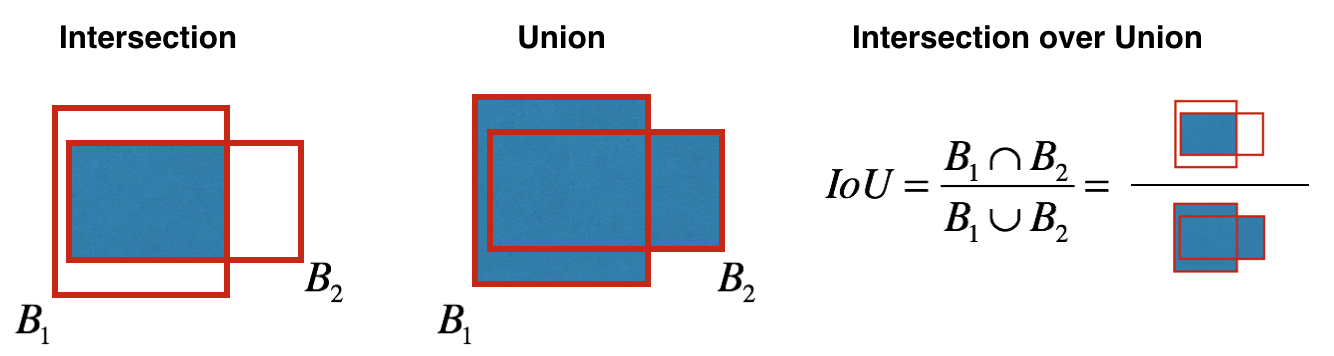
\includegraphics[width=0.5\textwidth]{Figures/IoU.png}
	\caption[Caption for figure in TOC.]{Diagram of the Intersection over Union (IoU) calculation, from~\cite{IoU_image_credit}}
	\label{fig:IoU}
\end{figure}

\subsection{Accuracy Metrics}
\label{sec:map}


The mean Average Precision (mAP) is a measure used to compare networks that use the Common Objects in
Context (COCO) dataset~\cite{coco:Microsoft}.

%FIX explanation
%The mAP metric gives an indication of the degree to which the correct
%classification have the highest confidence levels.
%???(FIXED) - isto não esta aqui a fazer nada, mas vale nao confundir


The mAP is the average of the
AP calculated for each class. The AP is calculated by ordering the
classifications performed by the highest bounding box confidence level. The
classifications are evaluated as true positives or false positives according to the ground truth. At each classification is also calculated the precision and recall, given by
\begin{equation}
	recall = \frac{\#True \ Positives}{\# Total True Positives} \text{ and } precision = \frac{\# True \ Positives}{\# Classifications}.
	\label{eq:precision_recall}
\end{equation}
The true positives are the number of correct classifications up to the classification being analysed and the total true positives are the total number of objects in the image. The number of classifications corresponds to the order of the classification being analysed. A precision/recall curve is calculated with the values computed for each classification as is presented by the orange curve in Fig.~\ref{fig:mAP}. The curve is then altered in order to have monotonically decreasing precision, by setting the precision at a given point equal to the maximum precision for any value of higher recall, as is presented by the green curve in Fig.~\ref{fig:mAP}. Finally, the AP is calculated by computing the area under the green curve.
%The mAP is the average of the
%AP calculated for each class. The AP is calculated by ordering the
%classifications performed by the highest bounding box confidence level. The
%classifications are evaluated as true positives or false positives according to the ground truth. From each
%true positive found onwards, the classifications receive the score of the recall
%at the true positive.
% how to decide if true or false?
\begin{figure}[!htb]
	\centering
	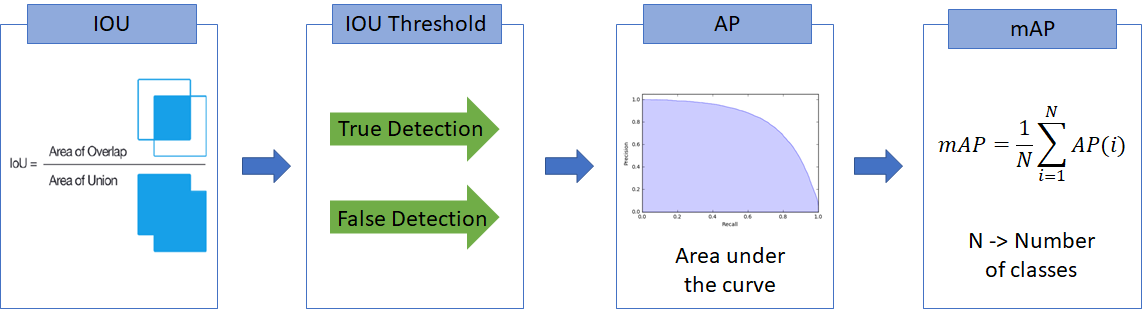
\includegraphics[width=0.5\textwidth]{Figures/mAP.png}
	\caption[Caption for figure in TOC.]{Example of precision/recall curve, adapted from~\cite{mAP}}
	\label{fig:mAP}
\end{figure}

%The score of classification $k$ is defined as interpolated
%precision ($P_{inter}(k)$).
%
%%how to compute Pinter ?
%
%
%With the number of ground truth positives (GTP), the
%AP is calculated by
%
%%what is GTP?
%
%\begin{equation}
%AP = \frac{1}{GTP} \sum_{i = 0}^{N} P_{inter}(i),
%\label{eq:AP}
%\end{equation}
%%END FIX (FIXED) - acabei por adicionar uma imagem, para mim é 1000x melhor do que qualquer texto que eu escreva
%where N is the total number of classifications above the IoU level.

Tab.~\ref{tab:yolov3_performance_metrics} presents the mAP
for a 0.5 IoU threshold and respective inference time (in ms) for
multiple networks. The results were obtained using machines with an M40 or Titan
X Pascal GPUs~\cite{yolov3} as indicated. The results show that the
Yolov3 networks achieve an accuracy on pair with the best performing networks at
a fraction of their inference time. The different versions of the Yolov3
networks are related with the resolution of the input images, but all have the
network structure.

\begin{table}[!htb]
	\renewcommand{\arraystretch}{1.2} % more space between rows
	\centering
	\begin{tabular}{lcccc}
		\toprule
		Network           & $mAP_{50}$ & Time (ms) & FPS & GPU  \\
		\midrule
		SSD321		& 45.4	& 61 & 16.4 & M40\\
		DSDSD321	& 46.1	& 85 & 11.8& M40\\
		R-FCN		& 51.9	& 85 & 11.8& M40\\
		SSD513		& 50.4	& 125 & 8& M40\\
		DSSD513		& 53.3	& 156 & 6.4& M40\\
		FPN FRCN	& \textbf{59.1} & 172 & 5.8& M40\\
		RetinaNet-50-500 & 50.9	& 73 & 13.7& M40\\
		RetinaNet-101-500 & 53.1	& 90 & 11.1& M40\\
		RetinaNet-101-800 & 57.5	& 198 & 5.1& M40\\
		Yolov3-320 & 51.5	& \textbf{22} & \textbf{45.5}& Titan X Pascal\\
		Yolov3-416 & 55.3	& 29 & 34.5& Titan X Pascal\\
		Yolov3-608 & 57.9	& 51 & 19.6& Titan X Pascal\\
		\bottomrule
	\end{tabular}
	\caption[Table caption shown in TOC.]{mAP and inference time comparison between multiple networks, adapted from~\cite{yolov3, Focal_Loss}.}
	\label{tab:yolov3_performance_metrics}
\end{table}

\subsection{Yolov3}
\label{sec:yolov3}
As presented in Tab.~\ref{tab:yolov3_performance_metrics}, the Yolov3 network
performs object detection at a higher framerate than other networks, while
maintaining a comparable level of accuracy.

\begin{table}[!htb]
	\renewcommand{\arraystretch}{1.2} % more space between rows
	\centering
	\begin{tabular}{lc}
		\toprule
		Layer Type           & Number of Layers  \\
		\midrule
		Convolutional       & 75    \\
		Shortcut  			& 23     \\
		Route 			    & 4     \\
		Yolo  				& 3     \\
		Upsample 		    & 2     \\
		Total 				& 107 \\
		\bottomrule
	\end{tabular}
	\caption[Table caption shown in TOC.]{Yolov3 layer type composition.}
	\label{tab:yolov3_num_layers}
\end{table}
Tab.~\ref{tab:yolov3_num_layers} presents the layer composition of the Yolov3
network. The majority of the layers are convolutional. Most of the convolutional
layers are used for feature detection or for reducing the FM resolution. This network
uses convolutional layers with $3\times3$ kernels with stride 2 instead of
pooling layers.

Due to the depth of the network, shortcut layers are used, to tackle the
problems described in section ~\ref{subsection:shortcut_layer}.

The accuracy performance for small object detection also comes from using three
different cell grid scales as opposed to the two used in previous
versions~\cite{Yolov2_redmon2016yolo9000}: ($13\times13$), ($26\times26$) and
($52\times52$). The indicated resolutions are specific to the Yolov3-416
version.

Fig.~\ref{fig:yolov3_stages} presents the main stages that constitute recurring
sequences of layers in the network: the F stage presented in
Fig.~\ref{fig:F_Stage} and the Yolo stage presented in
Fig.~\ref{fig:Yolo_Stage}.

\begin{figure}[!htb]
	\begin{subfigmatrix}{2}
		\subfigure[F stage composition]{\label{fig:F_Stage} 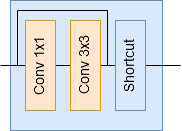
\includegraphics[width=0.25\textwidth]{Figures/FStage.png}}
		\subfigure[Yolo stage composition]{\label{fig:Yolo_Stage} 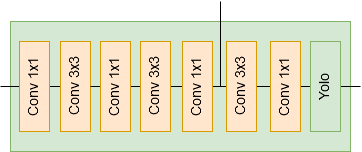
\includegraphics[width=0.50\textwidth]{Figures/YoloStage.png}}	
	\end{subfigmatrix}
	\caption{Stages of Yolov3 Network}
	\label{fig:yolov3_stages}
\end{figure}

Each F stage is composed of a convolutional layer with $1\times1$ kernels followed by
another with $3\times3$  kernels. At the end of the stage there is a shortcut layer
that adds the outputs of the second layer to the input of the stage.

In each Yolo stage, there is a sequence of convolutional layers, with $3\times
3$ and $1\times 1$ kernels that generate FMs of size $13 \times 13$ into the
first yolo layer. Since Yolov3 performs three detection attempts per grid cell,
there are $3\times 85 = 255$ FMs as input for every yolo layer. The
classification takes place for a grid with the same size as the FMs and the
number of FMs corresponds to the number os parameters to be calculated per grid
cell.

A complete scheme of the network is presented in Fig.~\ref{fig:Yolov3_complete}.

\begin{figure}[!htb]
	\centering
	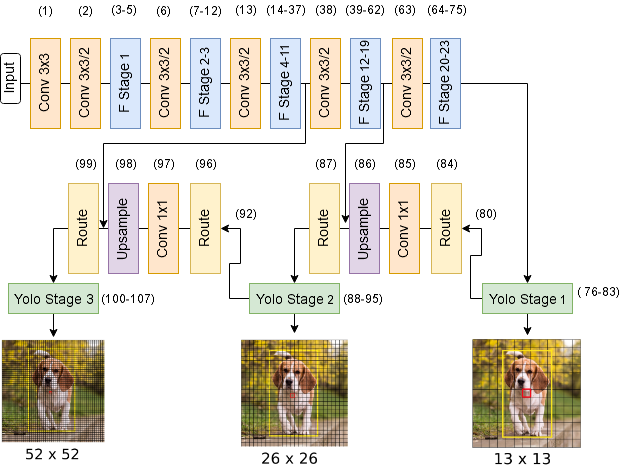
\includegraphics[width=0.85\textwidth]{Figures/CompleteYolov3Diagram.png}
	\caption[Caption for figure in TOC.]{Diagram of Yolov3 network}
	\label{fig:Yolov3_complete}
\end{figure}

The first part of the network is composed of a series of convolutional layers
terminated by F stages. Convolutional layers with stride 2 reduce the FMs by a
factor of four along the way. In this network implementation, the convolutions
use zero padding around the input FMs, so the size is maintained in the output
FMs. This part of the network is responsible for the feature detection in the
input image.

The second part of the netwok begins with a Yolo stage after which there is a
route layer that concatenates the output of the layers indicated in
Fig.~\ref{fig:Yolov3_complete}. This output is then compacted in terms of depth
by a $1\times 1$ convolution and upsampled by a factor of 2 in each FM
dimension, preparing the FMs for detections in a grid of $26\times26$ cells and
consequently detecting smaller objects in the image. These FMs are then
concatenated with the set of FMs of the same size from the detection part of the
network. The combination of the outputs of these two layers contribute with more
meaningfulness using the information from the upsampled layer and the
finer-grained information from the earlier feature maps~\cite{yolov3}.

After condensing the depth of the layer output to 255 FMs (again with a
convolutional layer with $1\times 1$ kernels), a second Yolo stage is used for
object detection at the new scale. The process is repeated one more time for the
third detection at the last yolo stage for a $52\times52$ grid.


\subsection{Tiny-YOLOv3}
\label{sec:tiny-yolov3}
For constrained environments, a small version of YOLOv3 is available. The layer
composition of the network is presented in
Tab.~\ref{tab:yolov3_tiny_num_layers}.

\begin{figure}[!htb]
	\begin{minipage}[b]{0.5\linewidth}
		\centering
		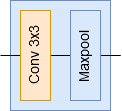
\includegraphics[width=0.35\textwidth]{Figures/TinyStage.png}
		\caption{Tiny-Yolov3 stage composition}
		\label{fig:Tiny_Stage}
	\end{minipage}%
	\begin{minipage}[b]{0.5\linewidth}
		\centering
		\begin{tabular}{lc}
			\toprule
			Layer Type           & Number of Layers  \\
			\midrule
			Convolutional       & 13    \\
			Maxpool  			& 6     \\
			Route 			    & 2     \\
			Yolo  				& 2     \\
			Upsample 		    & 1     \\
			Total 				& 24 \\
			\bottomrule
			
		\end{tabular}
		\caption[Table caption shown in TOC.]{Tiny-Yolov3 layer type composition.}
		\label{tab:yolov3_tiny_num_layers}
	\end{minipage}
\end{figure}

The first part of the network is composed of repeated Tiny-Yolov3 stages
presented in Fig.~\ref{fig:Tiny_Stage}. Each stage is composed of a
convolutional layer with $3\times3$ followed by a maxpooling layer.

This network follows the same sequence of layers present in Yolov3. The main
differences are in the number of layers and in the number of detections
performed. The Tiny-Yolov3 network performs object detection at only 2 grid
resolutions: $13\times13$ and $26\times26$.

\section*{Final Remark}
State-of-the-art CNN models are widely used for object detection
applications. These networks rely on convolution to extract features from the
images in order to be able to perform object detection. In order to achieve
higher performance metrics, CNNs grow in complexity. The Yolov3~\cite{yolov3}
network obtains comparable mAP for the COCO dataset~\cite{coco:Microsoft} to
other networks, at a fraction of the inference time.



 % file "Thesis_Background.tex"
\cleardoublepage

%%%%%%%%%%%%%%%%%%%%%%%%%%%%%%%%%%%%%%%%%%%%%%%%%%%%%%%%%%%%%%%%%%%%%%%%
%                                                                      %
%     File: Thesis_Implementation.tex                                  %
%     Tex Master: Thesis.tex                                           %
%                                                                      %
%     Author: João D. Lopes                                            %
%     Last modified :  7 July 2017                                     %
%                                                                      %
%%%%%%%%%%%%%%%%%%%%%%%%%%%%%%%%%%%%%%%%%%%%%%%%%%%%%%%%%%%%%%%%%%%%%%%%

\chapter{Architecture}
\label{chapter:architecture}

Versat is designed for fixed-point signal processing and its
architecture is shown in figure~\ref{fig_top}. It can be used by host
processors in the same chip, as some procedures can run faster and at
lower energy on Versat.

In order to reduce the dependency on the host CPU, Versat features a
simple Controller used for algorithmic control, self-reconfiguration
and data movement. This frees the host for more useful tasks. The
controller is programmable and has an instruction memory where Versat
programs (aka kernels) are stored. Control over the different modules
is exerted using a Control Bus. Though not shown, there is also a
serial divider accessible from the Control Bus.

Versat has a special unit that performs data computation, the Data
Engine (DE). This unit is composed of Functional Units (FUs)
interconnected by a full mesh. Hence, there is more than one way to
make a given datapath, which is useful for simplifying the compiler.

The Configuration Module (CM) holds the configuration of the DE, i.e.,
it specifies the current datapath, and has another register where the
next configuration of the DE can be prepared; it can also temporarily
store tens of other complete configurations, which can be switched at
runtime. The Controller can write partial configurations to the CM,
and can also save and restore entire configurations from the
configuration memory.

\begin{figure}[!htb]
\centering 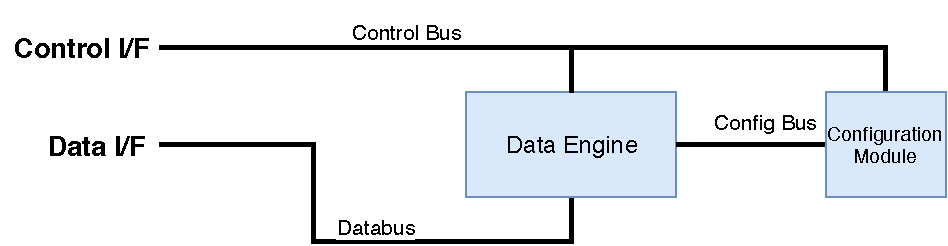
\includegraphics[width=0.70\textwidth]{drawings/top.pdf}
\caption{Versat top-level entity.}
\label{fig_top}
\end{figure}

Versat has a DMA module so it can independently and efficiently
transfer data, programs and configurations in and out of the
device. The DMA drives a master Advanced Extensible Interface --
AXI4. It is an interface designed by ARM, which derives from the
Advanced Microcontroller Bus Architecture (AMBA).

To communicate with the host processor, Versat has a shared Control
Register File (CRF). The CRF has two host interfaces that can be
selected at compile time: a Serial Peripheral Interface (SPI) and a
parallel bus interface. The SPI slave interface is used when the host
system is an off-chip master device. The SPI interface is mainly used
for debug and testing purposes. The parallel bus interface is used
when the host is some embedded processor and may be supplied in the
AXI4 Lite format.


%%%%%%%%%%%%%%%%%%%%%%%%%%%%%%%%%%%%%%%%%%%%%%%%%%%%%%%%%%%%%%%%%%%%%%%%
\section{Data Engine}
\label{section:dataEngine}

The Data Engine (DE) has a fixed topology comprising 15 Functional
Units (FUs) as shown in figure~\ref{fig_de}. The DE is a 32-bit
architecture and contains the following configurable FUs: 4 dual-port
embedded memories ($8kB$ each), 6 Arithmetic and Logic Units (ALUs), 4
multipliers and 1 barrel shifter. The output register of the FUs and
the embedded memories are accessible by the Controller for reading and
writing. (The embedded memory blocks are treated like any other FU by
the Versat tools.)

\begin{figure}[!htb]
\centering
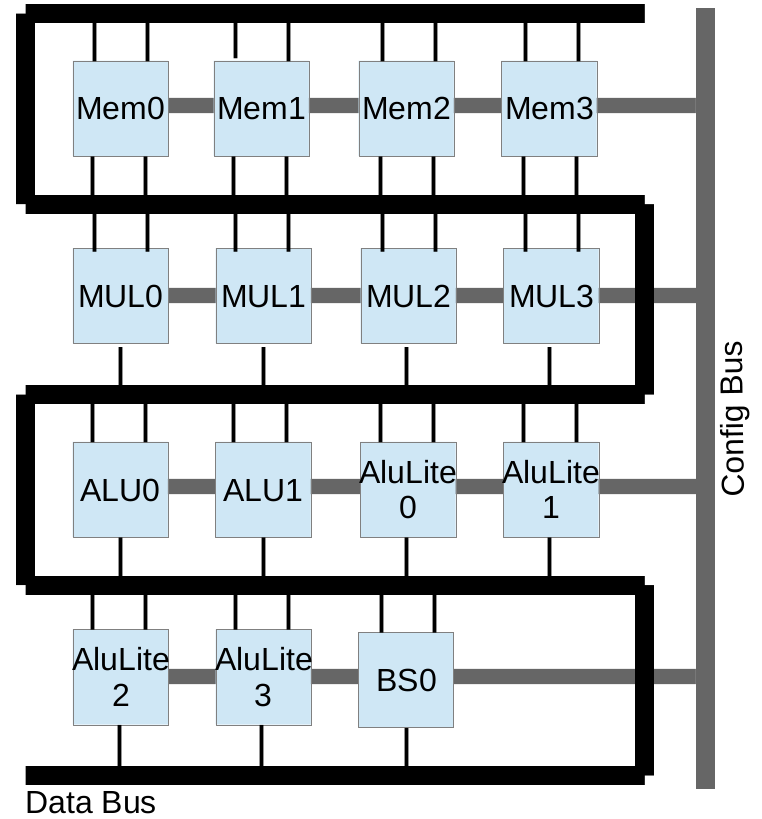
\includegraphics[width=0.75\textwidth]{drawings/de.pdf}
\caption{Data engine.}
\label{fig_de}
\end{figure}

\subsection{DE Structure}
\label{subsection:DEStructure}

In the DE, the FUs are interconnected by a wide bus called the Data
Bus. The Data Bus is simply the concatenation of all FU outputs. Each
FU output contributes a 32-bit section to the Data Bus, except the
embedded memories that contribute 2 sections with their 2
ports. According to the number of FUs of each type given before, the
Data Bus has $2\times4+6+4+1=19$ sections of 32 bits. In addition to
FU outputs, the Data Bus has 2 fixed sections containing the constants
0 and 1, which have been added because they are commonly used in
datapaths. Each FU input can select any of these sections and there is
also a selection that ignores the input value so that FU can be used
as a Controller shared register. The FUs take their configurations
from the respective configuration registers in the CM, whose outputs
are concatenated in another wide bus denoted the Config Bus. There is
a fixed set of high-level operations available in each FU. For
example, an ALU can be configured to perform addition, subtraction,
several logical functions, maximum, minimum, among others.

In figure~\ref{fig_fu}, it is shown in detail how a particular FU is
connected to the control, data and configuration buses. The FU, of
type ALU, is labeled FU5 and has 2 pipeline stages. The last pipeline
stage, denoted {\tt pipeline register 1}, stores the output of the
ALU, drives one section of the Data Bus and can be read or written by
the Controller using the Control Bus (as shown in the figure). This
feature enables the FUs to be used as Controller/DE shared
registers. Each FU5 input has a programmable multiplexer to select one
of the 19 sections of the Data Bus. Although the Config Bus is shown
going to all FUs, in fact only the configuration bits of each FU are
routed to it. These bits are called the {\em configuration space} of
the FU. The configuration space is further divided in several {\em
  configuration fields}, which are 3 in this example: the selection of
input A (5 bits), the selection of input B (5 bits) and the selection
of the function (4 bits). The partial reconfiguration scheme works at
the field level, so it is only possible to reconfigure these fields
individually.

\begin{figure}[!htb]
\centering
\includegraphics[width=0.85\textwidth]{drawings/FU.pdf}
\caption{Functional unit detail.}
\label{fig_fu}
\end{figure}

Since any FU can select any FU output as one of its inputs, then the
DE has a {\em full mesh topology}. This may seem exaggerated and
unnecessary but this topology accomplishes 2 major goals: (1) {\em an
  intuitive assembly programmer's model is achieved}; (2) {\em the
  compiler design is greatly simplified}. In fact, assembly
programmers need not remember or check what is connected to what since
everything is connected to everything. Hardware datapaths can be
manually built using store instructions that write to the
configuration fields of the used FUs. A compiler can be developed with
less effort as complex place and route algorithms, commonly used in
CGRAs, become unnecessary with a fully connected topology.

Assembly programmability is a powerful feature. It may be used to
optimize critical program sections or to work around bugs. In fact,
hardware bugs, defects or failures may eventually be circumvented at
post-silicon time using assembly code to avoid using the troubled
parts of the architecture. Compiler problems can also be fixed by
replacing the failing high-level code with assembly code.

In other approaches, such as in~\cite{Mei05}, a full mesh topology
would be problematic because of the cycle by cycle reconfiguration. It
causes frequent switching of the interconnect network and consequent
power dissipation. However, in Versat, reconfiguration does not happen
every clock cycle. The interconnect consumes very little power since
Versat is reconfigured only after a complete program loop or two
levels of nested loops are executed in the DE. It may also be argued
that a full mesh topology is large and limits the frequency of
operation. However, our IC implementation results indicate that only
$4.04\%$ of the core area is occupied by the full mesh interconnect,
while the core can work at a maximum frequency of $170MHz$ in a
$130nm$ process. This is sufficient for many target applications. For
example, in the multimedia space, some applications are required to
work at an even lower frequency because of power and energy
constraints.

Each configuration of the DE can implement one or more hardware
datapaths. Multiple datapaths operating in parallel realize
Thread-Level Parallelism (TLP). Datapaths having identical parallel
paths implement Data-Level Parallelism (DLP). Finally, datapaths
having long FU pipelines exploit Instruction-Level Parallelism (ILP).

In figure~\ref{fig_de_dp}, three example hardware datapaths are
illustrated. Datapath (a) implements a pipelined vector
addition. Despite the fact that a single ALU is used, ILP is being
exploited as the memory reads, addition operation and memory write are
being executed in parallel for consecutive elements of the
vector. Datapath (b) implements a vectorized version of datapath (a)
to illustrate DLP combined with the ILP. The vectors to be added
spread over memories M0 and M2, so that 2 additions can be performed
in parallel. ILP and DLP can be further exploited as in datapath (c),
whose function is to compute the inner product of two vectors: four
elements are multiplied in parallel and the results enter an adder
tree with an accumulator at the root. When an ALU is used as an
accumulator the unused data input is used as a control input. As seen
in the figure, this input is kept with the value 0, which specifies
the accumulator function. Any positive value specifies this function
while a negative value specifies that the ALU simply registers the
data input.

\begin{figure}[!htb]
\centering
\includegraphics[width=0.85\textwidth]{drawings/datapaths.pdf}
\caption{Data engine datapaths.}
\label{fig_de_dp}
\end{figure}


%%%%%%%%%%%%%%%%%%%%%%%%%%%%%%%%%%%%%%%%%%%%%%%%%%%%%%%%%%%%%%%%%%%%%%%%
\subsection{Address Generation Unit}
\label{subsection:addressGenerationUnit}

Versat has 4 dual-port Random Access Memories (RAMs) of size 2048
words by 32 bits, which work normally as vector registers. Each port
has an input, an output and an address input equipped with an Address
Generation Unit (AGU), as shown in figure~\ref{fig_dpram}. The AGUs
can be programmed to generate an address sequence for accessing data
from the memory port during the execution of a program loop. Our AGU
scheme is similar to the one described in~\cite{Farahini14}, in the
sense that both schemes use parallel and distributed AGUs. The AGUs
support two levels of nested loops, with the restriction that the
inner loop has a maximum of 32 iterations and the outer loop has a
maximum of 2048 iterations. To compute longer loops reconfiguration is
needed. AGUs can start execution with a programmable delay, so that
circuit paths with different accumulated latencies can be
synchronized. Each AGU can be operated independently from the other
AGUs, which allows TLP in the DE.

\begin{figure}[!htb]
\centering
\includegraphics[width=0.45\textwidth]{drawings/dpram.pdf}
\caption{Dual-port embedded memory with AGUs.}
\label{fig_dpram}
\end{figure}

Datapath (b) in figure~\ref{fig_de_dp}, previously used to explain
DLP, can also be used to explain TLP as follows. Suppose one block of
vector elements to be added is placed in memory M0, and that its
address generators M0-A, M0-B and M1-A are started (Thread 1). In
parallel, one can move the next block to memory M2 and start AGUs
M2-A, M2-B and M1-B (Thread 2). The user program can monitor the
completion of these threads and restart them with new vector
blocks. In this way, vectors that largely exceed the capacity of the
DE memories can be processed in a continuous fashion.

\begin{table}[!htb]
  \renewcommand{\arraystretch}{1.2} % more space between rows
  \caption{Address generation unit parameters.}
  \label{tab:MemParameter}
  \centering
  \begin{tabular}{lcp{10cm}}
    \toprule
    Parameter & Size (bits) & Description\\
    \midrule
    Start     &          11 & Memory start address. Default value is 0. \\
    Per       &           5 & Number of iterations of the inner loop, aka Period. Default is 1 (no inner loop). \\
    Duty      &           5 & Number of cycles in a period (Per) that the memory is enabled. Default is 1.\\
    Incr      &          11 & Increment for the inner loop. Default is 0.\\
    Iter      &          11 & Number of iterations of the outer loop. Default is 1.\\
    Shift     &          11 & Additional increment in the end of each period. Note that Per+Shift is the increment of the outer loop. Default is 0.\\
    Delay     &           5 & Number of clock cycles that the AGU must wait before starting to work. Used to compensate different latencies in the converging branches of the configured hardware datapaths. Default is 0.\\
    Reverse   &           1 & Bit-wise reversion of the generated address. Certain applications like the FFT work with mirrored addresses. Default is 0.\\
    \bottomrule
  \end{tabular}
\end{table}

The AGU parameters control the generation of address sequences and are
described in~Table~\ref{tab:MemParameter}. With these parameters the
AGU can generate an address sequence for an embedded memory port. An
example address sequence is shown in figure~\ref{fig_addrgen}. Note
that the AGU is enabled with a Delay of 2 clock cycles. It is enabled
periodically for $Duty=3$ cycles after every $Per=5$ cycles. The
initial value of the sequence is given by $Start=10$ (in decimal
notation). Every enabled cycle it is incremented by $Incr=2$; in the
last cycle of a period it is incremented by $Incr+Shift=-3$. This
pattern repeats for $Iter$ iterations, though this parameter is not
illustrated in the figure.

\begin{figure}[!htb]
\centering
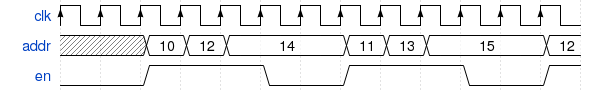
\includegraphics[width=0.75\textwidth]{drawings/addrgen.png}
\caption{AGU output for $Delay=2$, $Per=5$, $Duty=3$, $Start=10$, $Incr=2$, and $Shift=-5$.}
\label{fig_addrgen}
\end{figure}

The embedded memory ports have their own configuration fields: one for
selecting/disabling the input or outputting the generated sequence
(sel) and another for bypassing the AGU (Ext). If the input is
disabled then the port is enabled for reading. If it is selecting a
data source, then it is enabled for writing but also reads the word
previously stored at that address. Normally an AGU is used for
generating an address sequence for the memory port. However, the port
can also be configured to output the generated sequence to the DE,
where it can be used for general purposes. With this feature, data
patterns, synchronization and control signals can be generated for the
FUs. The configuration for bypassing the AGU ($Ext=1$) enables the
port to use as address values computed by datapath. In this case the
port address is input by the other port of the same memory. This
feature provides Versat with the capability of working with pointers.

In summary, the two memory ports can be independently configured to
read and/or write the memory, each memory port can be read/written with
an address sequence computed by the AGU or by some datapath in the
DE, and a memory configured for writing also reads the previously
stored word from the same address with one clock cycle of latency.

%%%%%%%%%%%%%%%%%%%%%%%%%%%%%%%%%%%%%%%%%%%%%%%%%%%%%%%%%%%%%%%%%%%%%%%%
\subsection{Arithmetic and Logic Unit}
\label{subsection:arithmeticLogicUnit}

There are two types of Arithmetic and Logic Units (ALUs), denoted Type
I and Type II: 2 Type I and 4 Type II. Both types have two inputs, A
and B, and an output Y.  A summary of the ALU operations is given in
Table~\ref{tab:AluOpers}. The ALUs have 4 configuration bits for the
operation field and thus can support 16 different operations.

\begin{table}[!htb]
  \renewcommand{\arraystretch}{1.2} % more space between rows
  \caption{ALU functions.}
  \label{tab:AluOpers}
  \centering
  \begin{tabular}{lll}
    \toprule
    Operation              &                Type I & Type II (w/ feedback)\\
    \midrule
    Logic OR               &           Y = A $|$ B & Y = Y $|$ B\\
    Logic AND              &            Y = A \& B & Y = Y \& B\\
    Logic XOR              &      Y = A $\oplus$ B & NA\\
    Addition               &             Y = A + B & Y = (A$<$0)? B: Y+B\\
    Subtraction            &             Y = B - A & Y = (A$<$0)? B: Y-B\\
    Multiplexer            &     Y = (A$<$0)? B: 0 & Y = (A$<$0)? B: Y\\
    Sign extend 8          &    Y = A[7]...A[7..0] & NA\\
    Sign extend 16         &  Y = A[15]...A[15..0] & NA\\
    Shift right arithmetic & Y = {A[31], A[31..1]} & NA\\
    Shift right logical    &   Y = {'0', A[31..1]} & NA\\
    Signed compare         &       Y[31] = (A$>$B) & Y[31] = (Y$>$B)\\
    Unsigned compare       &       Y[31] = (A$>$B) & NA\\
    Count lead zeros       &            Y = CLZ(A) & NA\\
    Signed maximum         &            Y=max(A,B) & Y = (A$<$0)? Y: max(Y,B)\\
    Signed minimum         &            Y=min(A,B) & Y = (A$<$0)? Y: min(Y,B)\\
    Absolute value         &             Y=$|$A$|$ & NA\\
    \bottomrule
  \end{tabular}
\end{table}

Type II ALUs use one of the configuration bits to create an internal
feedback loop from the output to input A. With the other 3 bits, Type
II ALUs can support 8 operations. If the feedback bit is set to '0',
these operations are the same as for Type I ALUs. If the feedback bit
is set to '1', the operation has input B and the current output as
operands. In this case, input A becomes available for runtime control
of the ALU, which is used for implementing conditional statements in
operations ADD, SUB, MUX, MIN and MAX. For instance, the addition
operation (ADD) can be turned into a conditional accumulate operation:
the ALU accumulates the values coming to input B, if input A is not
negative or simply registers input B otherwise. In another example,
the signed minimum operation can be used to detect and register the
minimum value among only certain elements of a sequence coming to
input B, by using input A as a data qualifier. Often, an AGU is used
to generate control sequences for the control input A of an ALU. The
type II ALU is an original way to enable conditional execution in the
DE.

%%%%%%%%%%%%%%%%%%%%%%%%%%%%%%%%%%%%%%%%%%%%%%%%%%%%%%%%%%%%%%%%%%%%%%%%
\subsection{Multiplier and Barrel Shifter}
\label{subsection:multiplierBarrelShifter}

The multiplier produces a 64-bit result from two 32-bit operands and
has two configuration parameters. One parameter allows selecting the
lower or higher 32 bits of the result. The other parameter forces the
multiply result to be left shifted by 1 bit. This configuration is
useful when operands are in the Q1.31 fixed-point format, which is
used in many DSP algorithms. By setting the first parameter to select
the high part of the result and the second parameter to left shift it
by 1, the multiplication of two Q1.31 operands also yields a Q1.31
result.

The barrel shifter can perform left and right shifts. Right shifts can
be configured as logical (no sign extension, feed '0' to the left) or
arithmetic (with sign extension). One configuration parameter
determines the shift direction (left or right) and another parameter
sets the right shift type (arithmetic or logic). In one input of the
barrel shifter is the value to be shifted and in the other input is
the shift size (0 to 31).

%%%%%%%%%%%%%%%%%%%%%%%%%%%%%%%%%%%%%%%%%%%%%%%%%%%%%%%%%%%%%%%%%%%%%%%%
\subsection{Functional Unit Latencies}
\label{subsection:functionalUnitLatencies}

Each FU has a latency due to pipelining: 2 clock cycles for the ALUs,
3 for the multipliers and 1 for the barrel shifter and embedded
memories. When configuring a datapath in the DE, it is necessary to
take into account the latency of each branch, and compensate for any
mismatches when branches with different latencies converge. To do
this, the AGUs have the {\em Delay} parameter explained in
Table~\ref{tab:MemParameter}. The branch latency is the sum of its FU
latencies.

%%%%%%%%%%%%%%%%%%%%%%%%%%%%%%%%%%%%%%%%%%%%%%%%%%%%%%%%%%%%%%%%%%%%%%%%
\subsection{Data Engine Control}
\label{subsection:dataEngineControl}

The DE is controlled using its Control and Status registers. The
Control register structure is the following: bit 0 (init) resets the
selected memory ports and bit 1 (run) enables the selected ports,
resets the selected FUs and starts the DE; bits~2~-~20 select the
memory ports and FUs to reset or enable. Recall there are 8 memory
ports and 11 other FUs in a total of 19 FUs to control. The Status
register structure is the following: bits~0~-~7 indicate which AGUs
are running (logic '0') or idle (logic '1').

%%%%%%%%%%%%%%%%%%%%%%%%%%%%%%%%%%%%%%%%%%%%%%%%%%%%%%%%%%%%%%%%%%%%%%%%
\section{Configuration Module}
\label{section:configuration}

The Configuration Module (CM) is composed of a Configuration Register
File used to prepare the next configuration, the Configuration Shadow
Register which holds the configuration being executed by the DE, and
the Configuration Memory where frequently used configurations are
stored (figure~\ref{fig_conf}). Configurations stored in the
configuration memory can later be used without modifications or they
can be partially reconfigured before used.

The configuration register file is divided in configuration spaces
which in turn are divided in configuration fields. Different
configuration spaces differ on the number of fields and configuration
fields differ on the number of bits. A full DE configuration is 672
bits. The configuration register file is addressable at the
configuration field level and there are 118 configuration fields. This
feature takes advantage of the fact that in most applications there is
a high likelihood that a certain configuration or a similar one will
be reused (time locality) to make partial reconfiguration effective.

The configuration shadow register holds an active configuration word
for the DE, which is copied from the configuration register file
whenever the Update signal is asserted by the Controller. Thus, the
contents of the configuration register file can be changed while the
configuration shadow register keeps the DE configured and running.

\begin{figure}[!htb]
\centering 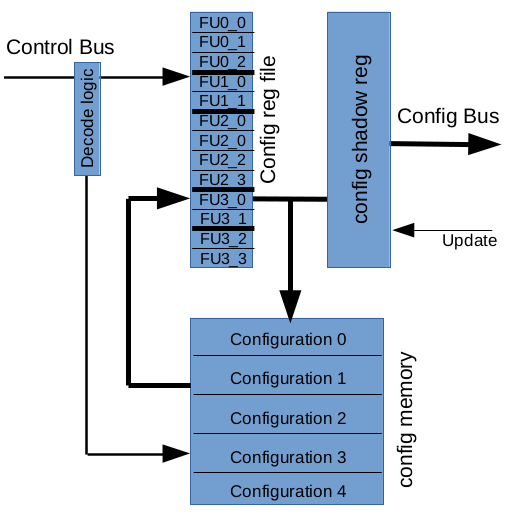
\includegraphics[width=0.8\textwidth]{drawings/conf.pdf}
\caption{Configuration Module.}
\label{fig_conf}
\end{figure}

The configuration memory is a dual-port 64-position memory, where each
position can store a full configuration and is, hence, 672 bits
wide. Configurations can be loaded/stored from/to the configuration
register file in just 1 clock cycle using one the memory ports. The
other port is 32-bit wide and used to load and store configurations in
the external memory using the DMA. This way, the configuration memory
can be extended beyond the 64 configurations. This scheme is designed
so that one can study the difference between working with pre-built
configurations stored in external memory and generating configurations
using the Versat controller.

%%%%%%%%%%%%%%%%%%%%%%%%%%%%%%%%%%%%%%%%%%%%%%%%%%%%%%%%%%%%%%%%%%%%%%%%
\section{Controller}
\label{section:controller}

The Versat Controller has a minimal architecture
(figure~\ref{fig_control}) to support reconfiguration, data movement,
algorithm control and host interaction. It contains 3 main registers:
the Program Counter (PC), the Accumulator Register (RA) and the
Address Register (RB). The PC contains the address of the next
instruction as usual. Register RA is the destination of all operations
that the controller performs, and is also often one of the operands
(accumulator architecture). Register RB is addressable by the
Controller and is used to store addresses for implementing indirect
loads and stores.

\begin{figure}[!htb]
\centering 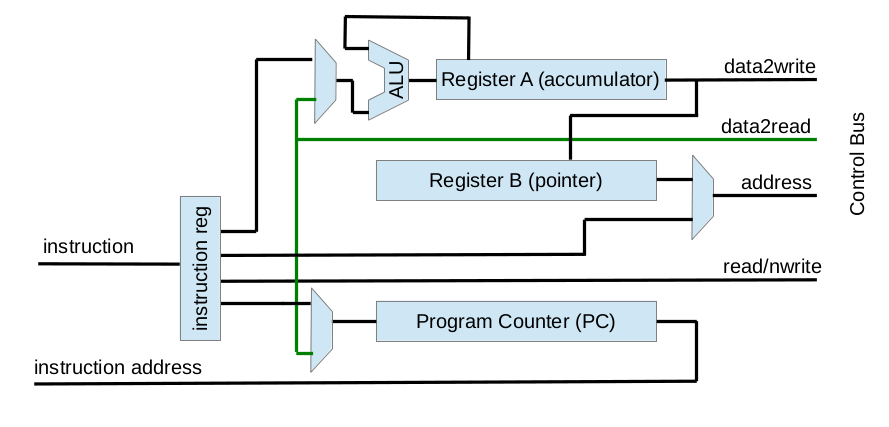
\includegraphics[width=0.95\textwidth]{drawings/control.pdf}
\caption{Controller.}
\label{fig_control}
\end{figure}

The controller has an instruction set of only 16 instructions ({\tt
  opcode} of 4 bits and {\tt Imm}ediate value of 16 bits). These allow
the controller to perform the following actions: loads/stores to/from
the accumulator, arithmetic/logic operations and branches. There are
three types of load instructions: of immediate constants, direct (from
an immediate address) and indirect from an address stored in register
RB. Store instructions can be direct or indirect.

The instruction set is outlined in Table~\ref{tab:isa}. As usual,
square brackets represent memory positions. For example, M[Imm]
represents the contents of the memory position whose address is
Imm. The PC is incremented for every instruction, except when
indicated otherwise (branch instructions).

\begin{table}[!htb]
  \renewcommand{\arraystretch}{1.2} % more space between rows
  \caption{Instruction set.}
  \label{tab:isa}
  \centering
  \begin{tabular}{cl}
    \toprule
    Instruction & Description\\
    \midrule
    nop   & No-operation\\
    rdw   & RA = M[Imm]\\
    wrw   & M[Imm] = RA\\
    rdwb  & RA = M[RB]\\
    wrwb  & M[RB] = RA\\
    beqi  & RA == 0? PC = Imm: PC += 1; RA = RA-1\\
    beq   & RA == 0? PC = M[Imm]: PC += 1; RA = RA-1\\
    bneqi & RA != 0? PC = Imm: PC += 1; RA = RA-1\\
    bneq  & RA != 0? PC = M[Imm]: PC += 1; RA = RA-1\\
    ldi   & RA = Imm\\
    ldih  & RA[31:16] = Imm\\
    shft  & RA = (Imm $<$ 0)? RA $<<$ 1: RA $>>$ 1\\
    add   & RA = RA + M[Imm]\\
    addi  & RA = RA + Imm\\
    sub   & RA = RA - M[Imm]\\
    and   & RA = RA \& M[Imm]\\
    \bottomrule
  \end{tabular}
\end{table}

In order to reduce the critical path and increase the clock frequency,
a pipeline register has been added between the instruction memory and
the instruction decoder. The controller then takes 2 clock cycles to
fetch an instruction, one from the memory itself and the other from
the instruction register shown in figure~\ref{fig_control}. For
simplicity, it executes every instruction fetched and thus branch
instructions have 2 delay slots. The delay slots can be filled with
useful instructions or with no operation (NOP) instructions.  For
instance, in a {\tt for} loop, the delay slots can be used to
increment the iteration count.

The boot loader software handles host procedure calls. The host writes
the procedure parameters to the CRF and writes the program address to
R0 which triggers a jump to the program address. During the execution
of a typical program, the DMA and the DE are used multiple times. DMA
and DE threads are spawned, hiding part of the controller execution
time, as shown later. This architecture allows programs to execute
precise time delays using a {\tt for} loop with a variable number of
instructions in its body. These instructions may be useful ones
(reconfiguration instructions, for instance) or just NOP instructions.

%%%%%%%%%%%%%%%%%%%%%%%%%%%%%%%%%%%%%%%%%%%%%%%%%%%%%%%%%%%%%%%%%%%%%%%%
\section{Divider}
\label{section:divider}

To perform divisions, Versat has a fixed-point serial divider, added
as a controller peripheral, which takes 33 cycles to complete one
division. It has shadow registers for the operands (dividend and
divisor), as well as for the results (quotient and remainder). This
means that it is possible to read the results and write next operands
while a new division is already being computed. It has one
configuration parameter that allows choosing between signed or
unsigned division. This implementation was designed for low energy and
small silicon area.

%%%%%%%%%%%%%%%%%%%%%%%%%%%%%%%%%%%%%%%%%%%%%%%%%%%%%%%%%%%%%%%%%%%%%%%%
\section{DMA}
\label{section:dma}

One of the crucial factors to guarantee acceleration is the rapidity
at which data is moved in and out of Versat. Accessing data words from
the external memory using load instructions is out of the
question. Data must be moved in large blocks using a DMA engine to
amortize the latency of the external memory device. The DMA engine is
operated by the Versat controller and transfers a data burst from
external memory into one of the Versat's memories (instruction,
configuration, or data engine memory) or vice versa.

From a Versat program point of view, the DMA is memory mapped and the
following DMA registers can be accessed: the external address
register, the internal address register, the size register, the
direction register, the status register and the start register. All
registers, except the status register, are duplicated allowing the
configuration of a new transaction while a previous one is
running. The external address register holds the transfer start
address in the external memory (32 bits), and the internal address
register holds the transfer start address in Versat (14 bits written
to a 32-bit register). The size register (8 bits) specifies the number
of words to be transferred (256 words maximum, as per the AXI4
interface). The direction register indicates if the transfer is from
Versat to external memory or vice-versa. After these registers have
been configured, the program writes anything to the start register and
the transfer begins. The contents of the status register tells the
program whether the DMA is still busy, done or if an error has
occurred.


%%%%%%%%%%%%%%%%%%%%%%%%%%%%%%%%%%%%%%%%%%%%%%%%%%%%%%%%%%%%%%%%%%%%%%%%
\section{Program memory}
\label{section:programMemory}

The Program Memory is divided in two parts: the boot ROM (256x32,
$1kB$) and the instruction memory RAM (2048x32, $8kB$). They are
addressable as a single memory: the first 256 addresses are used to
address the boot ROM, while the others are used to address the
instruction memory.

The boot ROM holds the code that allows Versat to communicate with the
host processor. Basically, it is used for the host to call Versat
kernels and to load/store values in any addressable memory position
within Versat without using the DMA. This includes loading programs
issuing store instructions to the Program Memory. However, the Program
Memory can not be read with load instructions. Its contents can only
be executed.


%%%%%%%%%%%%%%%%%%%%%%%%%%%%%%%%%%%%%%%%%%%%%%%%%%%%%%%%%%%%%%%%%%%%%%%%
\section{Control Register File}
\label{section:controlRegisterFile}

The 16x32 Control Register File (CRF) is implemented with a dual-port
register file (one port for the host and another for Versat). These
registers are shared between the host processor and Versat, which are
allowed to asynchronously read or write them.

\section{Qualitative comparison with other architectures}
\label{section:archComparisonWOtherArchitectures}

Versat has some distinctive features which can not be found in other
architectures: (1) it has a small number of FUs organized in a full
mesh structure; (2) it has a fully addressable configuration register
combined with a configuration memory to support partial configuration;
(3) it has a dedicated controller for reconfiguration, DMA management
and simple algorithm control -- no general purpose RISC~\cite{Lee00}
or VLIW~\cite{Mei05} processors are used.

CGRAs started as 1-D structures~\cite{Ebeling96} but more recently 2-D
square mesh FU arrays became more common~\cite{Lee00,Mei05,Liu15}. The
problem with square mesh topologies is that many FUs end up being used
as routing resources, reducing the number of FUs available for
computation and requiring sophisticated mapping
algorithms~\cite{Liu13}. Versat is an experiment on trading a lower FU
count with a richer interconnect structure. As explained before, the
silicon area occupied by the full mesh interconnect is less than $5\%$
and the limits placed on the frequency of operation are normally
irrelevant given the low energy budgets of target applications. In
fact, a low energy consumption often imposes a frequency of operation
which is well below Versat's maximum operating frequency.

As explained in~\cite{Liu15}, the reconfiguration time in CGRAs can
easily dominate the total execution time. To counter this effect
Versat takes partial reconfiguration to the extreme of using a fully
addressable configuration register. This keeps the reconfiguration
time to a minimum and contrasts with the more moderate hierarchical
reconfiguration scheme proposed in~\cite{Liu15}.

Since it is crucial to have reconfiguration done quickly, Versat
includes a small 16-instruction controller with low IO latency,
practically dedicated to reconfiguration management. This controller
is also used to manage data transfers and control the execution of
acceleration kernels. In other architectures~\cite{Lee00,Mei05,Liu15},
more comprehensive processors are used, which can also run complex
algorithms. However, combing complex application coding and
accelerator control is difficult. Using its controller, Versat can
completely take care of simple yet compute intensive kernels. Example
kernels are FFT, DCT, Motion Estimation, and even Big Data algorithms
such as K-Means Clustering. These kernels can simply be invoked by
host processors, and they will run in parallel to completion, without
requiring any external control.


\begin{comment}
After hardware reset the Versat, through boot ROM program, waits a
host command. Three registers of the CRF are used for this purpose:
one as a command register (R14), two as an address register (R0) and
another one as a data register (R15).

There are 3 commands (for now): read command, that allow the host to
access some data from Versat (for debug, for instance), write command,
that host uses to write some data into Versat, and run command, that
indicates to Versat to run some kernel.

In case of read, the host writes the read command into R14 (\#4), the
base address into R0 and waits that Versat write Acknowledge (Ack -
\#3) into R14. When it does, he read data from R15, clean Ack value
from R14 and waits for a new Ack. On Versat side, which is reading R0
until it has a nonzero value, after host command (written on R0), he
process the command given and get into a certain loop according the
command. In this case, after he loads the R0 value into RB, get into a
loop that reads R14 until it has a value that is not Ack. When this
happens, he checks if R14 value is equal to finish (\#2). If it is, go
back to boot ROM base address (cleans the R0 and wait it has a nonzero
value again), if not, read from the address pointed by RB, put the
data into R15, increment RB, write the Ack into R14 and go back to
read R14 loop (waits that R14 has a different value again).

In case of write, the host writes the first data value into R15, the
command into R14 and the base address into R0 (there is no write
command, it just have to be a different value that other commands uses
on protocol - i.e. \#0). When it does, he get into a loop that reads
R14 and wait for Ack. On Versat side, after processing the command
given, loads the R0 value into RB and get into a loop that reads R14
until it has a value that is not Ack. When this happens, he checks if
R14 value is equal to finish (\#2). If it is, go back to boot ROM base
address (cleans the R0 and wait it has a nonzero again), if not, write
R15 value into the address pointed by RB, increment RB, write the Ack
into R14 and go back to read R14 loop (waits that R14 has a different
value again).

For the execution of a kernel, the CRF is used by the host also to
pass parameters to Versat and by Versat to return status information
to the host (the registers used to do that are undefined, depends on
the kernel it self). After a host command, Versat do an unconditional
branch to address written on R0, starting the kernel execution.
\end{comment}
 % file "Thesis_Implementation.tex"
\cleardoublepage

%%%%%%%%%%%%%%%%%%%%%%%%%%%%%%%%%%%%%%%%%%%%%%%%%%%%%%%%%%%%%%%%%%%%%%%%
%                                                                      %
%     File: Thesis_Programming.tex                                     %
%     Tex Master: Thesis.tex                                           %
%                                                                      %
%     Author: João D. Lopes                                            %
%     Last modified :  20 September 2017                               %
%                                                                      %
%%%%%%%%%%%%%%%%%%%%%%%%%%%%%%%%%%%%%%%%%%%%%%%%%%%%%%%%%%%%%%%%%%%%%%%%

\chapter{Programming}
\label{chapter:programming}

Versat can be programmed using a C/C++ subset, and the code can be
compiled using the Versat compiler~\cite{Santiago2016}. Versat can
also be programmed in assembly language, given its easy to apprehend
structure. To the best of our knowledge, Versat is the only CGRA that
can be programmed in assembly. In this chapter, Versat programming is
illustrated using its C/C++ dialect, which is easier for explaining
the basic concepts. Also it will be explaind how to use Versat drivers
from the host system point of view (where the host system is an
embedded processor, for instance an ARM processor).

%The programming tools will not be explained as they are not the main focus of this report.

% ----------------------------------------------------------------------
\section{Basic programming}
\label{section:basicProgramming}

In order to outline the basics of Versat programming, a typical
example program is given in this section. The program adds two memory
interleaved vectors: one vector resides in the even addresses while
the other vector resides in the odd addresses. The program is shown in
figure~\ref{fig_vec_add} and comments are added for clarity.

\begin{figure}[!htb]
\centering \includegraphics[width=0.8\textwidth]{drawings/code.pdf}
\caption{Vector addition code.}
\label{fig_vec_add}
\end{figure}

The program starts in the {\tt main()} function, as is usual in C/C++
programs, and proceeds immediately to loading Versat with data using
the DMA. The DMA is configured ({\tt dma.config()}) with the external
and internal addresses, transfer size and direction. The {\tt
  dma.run()} function sets the DMA running, but does not wait for its
completion.

With the DMA running, the program proceeds to configure the DE. The
configuration register file is cleared in order to start a new
configuration ({\tt de.clearConfig()}). Certain language constructs
are interpreted as DE configurations and the compiler automatically
generates instructions that write these configurations to the CM. This
is the case of the ensuing {\tt for} loop. The fact that memory ports
are invoked in its body triggers this interpretation. Note that object
or variable declarations are not yet supported by the compiler. Data
must be referenced using the names of the memories or registers where
they are stored. When variables are supported, the issue of
recognizing DE configurations will need further research. For now, it
can be conjectured that the presence of data arrays in a loop is
sufficient for inferring a DE configuration. In the given example, the
expression in the loop body configures the DE to read the two vectors
from the two ports of memory 0, add their elements and place the
result in memory 1 using its port A.

Next, the program checks whether the DMA has finished loading the
data. The {\tt dma.wait()} function blocks the Controller until the
DMA is idle again. Note that the DMA has been running concurrently
with the Controller, which has been configuring the DE.

Once the DE is loaded and configured, it is run by means of the {\tt
  de.run()} function call. While it runs, the DMA is configured in
advance to transfer the result of the vector addition to the external
memory. Then the program waits for DE completion ({\tt de.wait()}) and
runs the DMA ({\tt dma.run()}). It is necessary to wait for DMA
completion ({\tt dma.wait()}) before exiting the program, to guarantee
that the result is stored in the external memory before control is
passed to a host processor.

% ----------------------------------------------------------------------
\section{Self and partial reconfiguration}
\label{section:selfPartialReconfiguration}

In this section, an example is presented to illustrate {\em
  self-generated partial reconfiguration} in Versat
(figure~\ref{fig_preconf}). The example shows a {\tt do-while}
loop. These kind of loops are always executed by the Controller,
because the DE has no means to stop conditionally.

\begin{figure}[!htb]
\centering \includegraphics[width=0.8\textwidth]{drawings/code2.pdf}
\caption{Self and partial reconfiguration code.}
\label{fig_preconf}
\end{figure}

A 2-level nested loop follows, where the body contains only
expressions involving memory ports. This nested loop is therefore
interpreted as a DE configuration and the compiler generates
instructions that write this configuration to the CM. Note that the
memory address expressions (between square brackets) use register R1,
which is updated inside the {\tt do-while} loop: R1 depends on R7
which is also updated in the loop.

In fact, R1 is the start address for the data in memories 0 and 1,
which corresponds to the Start parameter of the AGUs in the memory
ports used (see Table~\ref{tab:MemParameter}). Thus, only the Start
parameters in these AGUs need to be reconfigured, which means the DE
is {\em partially reconfigured} in each iteration of the {\tt
  do-while} loop.

Furthermore, the {\tt do-while} loop is {\em generating} one DE
configuration per iteration. Since this is done by the Controller,
without any intervention of the host processor, it may be said that
{\em Versat is self-reconfigurable}.

The {\tt de.wait()} function call, after the nested loop, waits for
the previous DE configuration to finish running. The following {\tt
  de.run()} function call runs the DE again for the current
configuration. While the DE is running, registers R7 and R12 are
updated and the {\tt do-while} loop goes on to the next iteration,
provided the loop control register (R12) is non-zero. In the next
iteration R1 is updated, the DE is partially reconfigured for the next
run, and the process repeats all over again.

% ----------------------------------------------------------------------
\section{Versat Driver}
\label{section:drivers}

Versat is designed to work as a co-processor for host systems. The
host system needs a very simple driver, which consists of only a few
functions for managing Versat. A program that uses the Versat driver
as is shown in the figure~\ref{fig_drivers}.

\begin{figure}[!htb]
\centering \includegraphics[width=0.8\textwidth]{drawings/drivers.pdf}
\caption{C code using Versat drivers.}
\label{fig_drivers}
\end{figure}

The reduced number of functions present in the driver make Versat very
easy to use by host processors. This is mainly because Versat is very
independent, it can reconfigure itself, access data from the external
memory and run simple control algorithms. However, Versat needs to be
programmed separately.

To use the driver, first of all, the header file ({\tt versat.h}) must
be included in the source file of the host program willing to use
Versat as an accelerator.

Second, the {\tt versat\_load()} function is called to load Versat
kernel(s) into Versat's program memory. Parameter {\tt progExt\_addr}
is the external memory address where the program resides and parameter
{\tt progInt\_addr} is the internal (to Versat) memory address where
it should be transferred; parameter {\tt progSize} is the kernel size
in 32-bit words.

Next, the {\tt versat\_wait()} function is called for waiting until
Versat has finished the last command. In this case, it guarantees that
the kernel code is already in the program memory, so that Versat is ready
to execute the next command.

Then, the {\tt versat\_run()} function is called to start execution. A
FFT kernel is used as the example. The first parameter, {\tt FFT},
identifies the kernel to be run. It is actually the address of the
kernel in Versat's program memory. Parameters {\tt x\_ptr}, {\tt
  w\_ptr} and {\tt X\_ptr} indicate the location of the input and
output vectors in the external memory. The FFT is computed over a
complex dataset of {\tt Npts} points, using windows of size {\tt
  WindowSize}, where two consecutive windows overlap by {\tt Overlap}
points.

While Versat is running, some host code could be put before calling
the {\tt versat\_wait()} function again, as this code will execute in
parallel with Versat if it does to take more time than the Versat
kernel. When the {\tt versat\_wait()} function exits the FFT
computation is done and one may add some post-processing code before
exiting the host program.


% ----------------------------------------------------------------------
\section{Comparison with other architectures}
\label{section:progComparisonWOtherArchitectures}

Versat is the only known CGRA that can be programmed in assembly
language. It supports configurations pre-compiled, i.e., is capable of
using configurations that are stored in the external memory, by
transferring them into its own configuration memory like other
architectures that can only be full reconfigured by transferring
configurations~\cite{Lee00,Mei05,Hartenstein99}. As it is able to
perform {\em self and partial reconfiguration}, i.e., generate
configurations on the fly and use highly sophisticated reconfiguration
mechanisms to partially modify them, since they use to be similar to
each other. Unlike some other architectures that use inefficient
reconfiguration mechanisms and some of them are very recommended not
be used~\cite{Ebeling96,Weinhardt03,Liu15}.

In conclusion, Versat is a very capable architecture of perform {\em
  self and partial reconfiguration} on the fly. It works as a
co-processor used to accelerate data computation, attached to a host
system who calls it by using some procedures stored in the Versat's
library ({\tt versat.h}). It is quite independent from the host system
for generating configurations and transfer the data to/from the
external memory, freeing the host for other useful computations.
 % file "Thesis_Programming.tex"
\cleardoublepage

%%%%%%%%%%%%%%%%%%%%%%%%%%%%%%%%%%%%%%%%%%%%%%%%%%%%%%%%%%%%%%%%%%%%%%%%
%                                                                      %
%     File: Thesis_Applications.tex                                    %
%     Tex Master: Thesis.tex                                           %
%                                                                      %
%     Author: João D. Lopes                                            %
%     Last modified :  18 April 2017                                   %
%                                                                      %
%%%%%%%%%%%%%%%%%%%%%%%%%%%%%%%%%%%%%%%%%%%%%%%%%%%%%%%%%%%%%%%%%%%%%%%%

\chapter{Applications}
\label{chapter:applications}

The Versat architecture is suitable to be used in ultra low energy
applications such as those found in Wireless Sensor Networks (WSNs),
where using a GPU or FPGA accelerator is out of the question. A
dedicated hardware accelerator may also be used but its lack of
programmability can become a serious liability in the long run. In
this chapter, two algorithms that can be used in such applications are
presented: the Fast Fourier Transform and the K-Means Clustering
algorithms. Their implementation on Versat demonstrates the
versatility of the architecture.

% ----------------------------------------------------------------------
\section{Fast Fourier Transform }
\label{section:FFT}

The Fast Fourier Transform (FFT) is an algorithm for efficiently
computing the Discrete Fourier Transform (DFT) of a digitized
signal. It is used in many signal processing applications such as
filters, audio and video pre and post processing, as well as encoders
and decoders (spectral analysis in general). There are many
implementations of the FFT algorithm. In this work, the Radix-2 FFT
algorithm has been chosen, due to its simplicity. In the next subsection,
a formal description of the DFT is presented, and in the subsection
after, the Cooley-Tukey Radix-2 FFT algorithm is described.

% ----------------------------------------------------------------------
\subsection{Discrete Fourier Transform}
\label{subsection:DFT}

The Discrete Fourier Transform $X(k)$ of a discrete signal $x(n)$
having $N$ samples is given in the following equation
\begin{equation}
X(k)=\sum_{n=0}^{N-1} W_N^{kn}x(n),\ \ 0\leq k\leq N-1,
\label{eq:DFT}
\end{equation}
where the coefficients $W_N^k$ are given by
\begin{equation}
W_N^k=e^{-j\frac{2\pi k}{N}}.
\label{eq:DFTcoefficients}
\end{equation}

The most obvious way to compute $X(k)$ is to perform $N$ complex
multiplications ($4N$ real multiplications plus $2N$ real additions)
and $N-1$ complex additions ($2N-2$ real additions). Because one needs
to compute $N$ points of the DFT, the algorithm complexity is
$O(N^2)$. Attending to the coefficients symmetry
(equation~\ref{eq:coeffSymmetry}) and periodicity
(equation~\ref{eq:coeffPeriod}), it is possible achieve a better
algorithm, and the Cooley-Tukey FFT Algorithm, explained in the next
subsection, is just that.

\begin{equation}
W_{N}^{k+\frac{N}{2}}=-W_{N}^{k}
\label{eq:coeffSymmetry}
\end{equation}

\begin{equation}
W_{N}^{k+N}=W_{N}^{k}
\label{eq:coeffPeriod}
\end{equation}

%The one that was chosen was the Cooley-Tukey algorithm, because it is
%the most commonly used. % reference

% ----------------------------------------------------------------------
\subsection{Cooley-Tukey Algorithm}
\label{subsection:CooleyTukeyAlgorithm}

The DFT computation for $N$ points can be decomposed in two independent
DFT computations of $N/2$ points, for $N$ even, separating the points
which have even indices from the ones that have odd
indices. Equation~(\ref{eq:DFT}) can thus be rewritten as
\begin{equation} 
  X(k) = \sum_{n=0}^{(N/2)-1} W_N^{k(2n)} x(2n) + 
  \sum_{n=0}^{(N/2)-1} W_N^{k(2n+1)} x(2n+1).
  \label{eq:splitDFT}
\end{equation}

From equation~(\ref{eq:DFTcoefficients}) it can be derived that
$W_N^{2k} = W_{N/2}^k$ and equation~(\ref{eq:splitDFT}) can be rewritten as
\begin{equation}
X(k)=\sum_{n=0}^{(N/2)-1} W_{N/2}^{kn} f_e(n) + W_N^k \sum_{n=0}^{(N/2)-1} W_{N/2}^{kn} f_o(n),
\label{eq:splitDFT2}
\end{equation}
where $f_e(n) = x(2n)$ and $f_o(n)= x(2n+1)$. Hence,
equation~(\ref{eq:splitDFT2}) can be written as
\begin{equation} 
X(k)=F_e(k)+W_N^k F_o(k), \ \ 0\leq k\leq N-1.
\label{eq:DFTdecomp}
\end{equation}

Since $F_e(k)$ and $F_o(k)$ are periodic with period $N/2$ and taking
into account the coefficients' symmetry, according to
equations~(\ref{eq:coeffSymmetry}) and~(\ref{eq:coeffPeriod}), the
previous expression can be rewritten as
\begin{equation}
\begin{split}
X(k) & =  F_e(k)+W_n^k F_o(k), \\
X \left ( k+\frac{N}{2} \right ) & =  F_e(k)-W_n^k F_o(k), \ \ 0\leq k\leq \frac{N}{2}-1.
\end{split}
\label{eq:DFTdecomp2}
\end{equation}

Equation~(\ref{eq:DFTdecomp2}) proves that it is possible to decompose
an $N$-point DFT into a weighted sum of {\em two} $N/2$-point
DFTs. This procedure can be applied recursively until the simplest
case of a 2-point DFT is reached. This happens after $log_2(N)$
recursion levels, which explains why this FFT algorithm is called {\em
  Radix-2}. In this algorithm there are $(N/2)log_2(N)$ complex
multiplications and $Nlog_2(N)$ complex additions. Therefore, the
Cooley-Tukey algorithm has complexity $O(Nlog(N))$.

A 2-point FFT computed in this way is shown in
figure~\ref{fig:FFTButterfly}. This is called a butterfly diagram
because of its shape. The input data is on the left, while the output
data is on the right. All data are complex numbers. The edges
represent the data flow. The edges apply the following weights to the
data: $W_N$, $-1$ or $1$ (by omission). Where edges merge, their
corresponding values are added. For optimization, an edge having the
coefficient $-1$ is simply subtracted from the other merging edge.

\begin{figure}[!htb]
	\centering{
      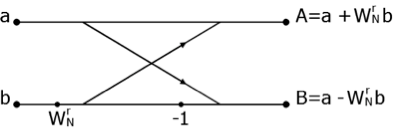
\includegraphics
            [width=0.5\columnwidth]
            {drawings/fftButterfly.png}
	}	
	\caption{Butterfly diagram.}
	\label{fig:FFTButterfly}
\end{figure}

A graphical example of the Cooley-Tukey algorithm applied to an
8-point signal $x$ is shown in figure~\ref{fig:FFT8pts}. The recursion
levels map to stages. In this example, there are $log_2(8)=3$
stages. Each stage has distinctive groups of butterflies called
blocks. The first stage has 4 blocks of a single butterfly, the second
stage has 2 blocks of 2 butterflies and the third stage has a single
block of 4 butterflies.

\begin{figure}[!htb]
	\centering{
      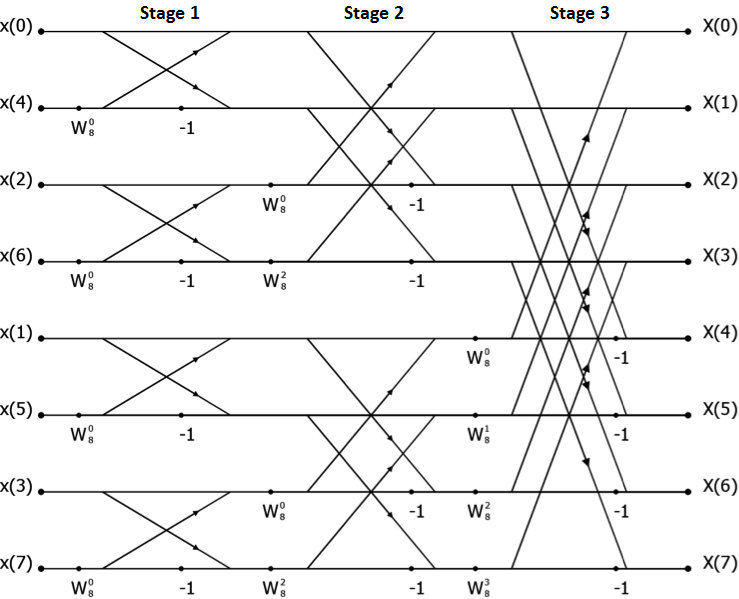
\includegraphics
            [width=0.8\columnwidth]
            {drawings/fft8pts.png}
	}	
	\caption{Cooley-Tukey agorithm appled to an 8-point signal $x$.}
	\label{fig:FFT8pts}
\end{figure}

The Versat FFT kernel implements the Cooley-Tukey algorithm by
splitting a basic butterfly structure in two steps:
\begin{enumerate}
	\item Complex multiplication step: the datapoints stored
          at odd addresses are multiplied by the coefficients
	\item Complex addition step: the datapoints stored at even
          addresses are added and subtracted from the results of the
          first step to yield 2 result datapoints
\end{enumerate}

% ----------------------------------------------------------------------
\subsection{Implementation}
\label{subsection:FFTImplementation}

The FFT kernel follows the algorithm given in the previous subsection,
creating and partially reconfiguring two basic hardware datapaths that
realize the {\em complex multiplication} and {\em complex addition}
steps of the algorithm. In fact, two versions of each datapath have
been created to enable ping-pong data processing. Another datapath is
used to initially reorder the datapoints by reverting the bits of
their addresses. The data format is 32-bit fixed-point in a Q1.31
organization. The kernel is written in the Versat assembly language
and it is 873 instructions long.

The datapath to initially reorder the data is shown in
figure~\ref{fig:mirrorAddresses}. The AGUs of the source memories MEM2
and MEM3 (port A) read the datapoints with the Reverse parameter set
to '1' (table~\ref{tab:MemParameter}), and the AGUs of the destination
memories MEM0 and MEM1 (ports A) write them
sequentially. Concurrently, the table of coefficients is copied from
MEM2 to MEM0 (ports B), so that either can be accessed during the
ping-pong processing.

\begin{figure}[!htb]
\centering
\includegraphics[width=0.8\columnwidth]{drawings/fft-mirrorAddresses.pdf}
\caption{Datapath for read the initial datapoints with mirrored
  addresses.}
\label{fig:mirrorAddresses}
\end{figure}

The Versat controller plays an important role in complex kernels like
the present FFT kernel. It is responsible for generating the
datapaths, reconfiguring them and controlling the algorithm. Namely,
it controls the outer loops over all stages and, in some cases, over
all blocks in a stage.

First, the four datapaths are created and stored in the configuration
memory. They are very similar two by two, swapping only the memories
that are used for reading with the ones that are used for storing the
data. This is done while data is being DMA transferred into the DE.

After reading a number of parameters from the CRF (number of
datapoints, window and overlap sizes and addresses to read/write data
in the external memory), as passed by the host, the program instructs
the DMA to load the first datapoint chunk values in memories MEM2 and
MEM3. Real parts go into MEM2 and imaginary parts into MEM3, not
exceeding the 1024 lower addresses. Coefficient values are also DMA
transferred into memory MEM2, occupying at most the 1024 higher
addresses. Then the data is reordered and placed in memories MEM0 and
MEM1 while the coefficients are copied to MEM0, using the reordering
datapath explained before.

The datapath in figure~\ref{fig:complexMultiplication} implements the
complex multiplication step, reading the data from MEM0 (real part)
and MEM1 (imaginary part) and coefficients from MEM2 (real and
imaginary parts), and writing the result back in MEM0 and MEM1. Its
configuration is loaded from the configuration memory into the
configuration register file in one clock cycle, partially
reconfigured, and shifted to the shadow configuration register in
another cycle. The datapath forms a read-multiply-add-write pipeline
with four multiplications and two additions in parallel in the
respective stages, combining DLP and ILP.

\begin{figure}[!htb]
\centering \includegraphics[width=0.85\columnwidth]{drawings/fft-cmult.pdf}
\caption{Datapath for the complex multiplication step.}
\label{fig:complexMultiplication}
\end{figure}

Next, the datapath that performs the complex addition step, shown in
figure~\ref{fig:complexSum}, is loaded. This datapath performs the two
complex additions in the butterfly diagram of
figure~\ref{fig:FFTButterfly}. Note that MEM0 (real part) and MEM1
(imaginary part) have the original data in the even addresses and the
original data multiplied by the coefficients in the odd
addresses. Therefore the data in the even addresses is added and
subtracted to the data in the odd addresses to produce the two
butterfly outputs. The results are placed in MEM2 (real part) and MEM3
(imaginary part). The parallel additions exploit DLP while the
read-compute-write pipeline exploits ILP.

\begin{figure}[!htb]
\centering \includegraphics[width=0.85\columnwidth]{drawings/fft-csum.pdf}
\caption{Datapath for the complex addition step.}
\label{fig:complexSum}
\end{figure}

After both steps are run, the controller increments the outer loop and
the two steps are applied again, now from MEM2 and MEM3 to MEM0 and
MEM1. This process is repeated until all stages are processed. Every
time the kernel needs more data, the current results are stored in the
external memory and new datapoints are loaded into the DE memories.

Because AGU parameter Period has only 5 bits
(table~\ref{tab:MemParameter}), there is need to break the two step
computations in several parts for some stages. This is because the two
nested loops that can be executed in the DE are used to go over all
blocks and all datapoints within a block. If there are more than
$2^5=32$ butterflies within a block then the inner loop cannot be
used. Only the iterations loop is used and the DE needs to be
reconfigured for each block. In order to save reconfiguration time,
the controller uses partial reconfiguration. Additionally, if an FFT
window cannot fit into the DE memories, the FFT computation is divided
into several smaller FFTs and several other steps to merge the
results.

After all stages are processed, the controller instructs the DMA to
transfer the results to the external memory, using the respective
address in the CRF passed by the host. Then, a new datapoint chunk is
loaded and the whole process starts again, until all datapoints are
processed and stored in the external memory. When this happens, the
algorithm terminates. Before returning to the boot ROM memory, the
controller clears register R0 in the CRF, which signals the host that
Versat has finished execution.

% ----------------------------------------------------------------------
\section{K-Means Clustering}
\label{section:kmeans}

The K-Means algorithm is one of the simplest algorithms for performing
the clustering task. Despite its simplicity, it is still one of the
most widely used clustering algorithms, due to its ease of
implementation and fast execution time.

% ----------------------------------------------------------------------
\subsection{Algorithm}
\label{subsection:kmeansAlgorithm}

The algorithm uses a centroid model. It separates the data into a set
of clusters, each having a centroid represented by the mean vector of
all the datapoints in the cluster. Each datapoint is classified as
being in the cluster whose centroid is closest to it. The Euclidean
distance is a common metric, though other types of metrics can be
applied~\cite{Estlick2001}. For simplicity, the Manhattan Distance
(MD) is used. After an initial position is given to each centroid, the
algorithm starts updating the position of the centers in an iterative
fashion. Each iteration is divided in two main steps:
\begin{enumerate}
	\item Assignment step: each datapoint is assigned to the
          nearest centroid, given the chosen distance metric
	\item Update step: the centroids are recalculated; the new
          positions correspond to the mean of all the datapoints in
          each cluster
\end{enumerate}
The algorithm ends when the centers are unchanged after an iteration.

% ----------------------------------------------------------------------
\subsection{Implementation}
\label{subsection:kmeansImplementation}

The K-Means Clustering kernel follows the algorithm given in the
previous subsection, creating and partially reconfiguring the two
basic hardware datapaths that realize the {\em assignment} and {\em
  update} steps of the algorithm. The kernel is written in the Versat
assembly language and it is 691 instructions long.

As happens in the FFT kernel, the two datapaths are created and stored
in the configuration memory. This is done while the first chunk of
data is being transferred into the DE by the DMA. After reading the
number of points, coordinates, centroids and respective external
memory addresses from the CRF, as passed by the host, the program
instructs the DMA to load the first datapoint chunk and initial
centroid values in memories MEM0 and MEM1, respectively. The datapoint
chunk size cannot exceed 2048x32bits, the size of MEM0 (starting at
the lower address). The number of centroids times the number of
coordinates is limited to 1024x32bits, half the size of MEM1 (starting
at the second half). The other half is reserved for incrementally
building the updated centroids. This is a hard limitation of this
algorithm, which can only be overcome by using a larger embedded
memory for the centroids, which costs silicon, or by streaming the
centroids as done with the datapoints, which penalizes
performance. However, in the target WSN applications, only a few
centroids are used, making the current algorithm implementation
acceptable.

\begin{figure}[!htb]
\centering \includegraphics[width=0.85\textwidth]{drawings/kmeans.pdf}
\caption{Datapath for the assignment step.}
\label{fig:assignment}
\end{figure}

The datapath in figure~\ref{fig:assignment} implements the assignment
step. Its configuration is loaded from the configuration memory into
the configuration register file and shifted to the shadow
configuration register in two clock cycles, as in the FFT kernel. The
DE is started and the first point is compared with all the centroids,
coordinate after coordinate. The absolute value of the coordinate
difference is accumulated in the type II ALU, configured with the {\em
  ACC if A} function. In this function, the A input instructs the ALU
to either store the first absolute difference or accumulate the
following ones. Input A is produced by the AGU from port B of MEM1,
which is thus not used to generate memory addresses -- this is on of
Versat's novel feature as explained in
section~\ref{section:dataEngine}. If $A < 0$ then the ALU stores,
otherwise it accumulates. After processing all coordinates, the MD is
ready. The ALU configured as {\em MIN if A} checks whether the current
centroid is the closest yet to the datapoint, by computing the minimum
between the current MD and the previous minimum. Input A is generated
by port B of MEM2 to synchronize this action. The current MD is
delayed by 1 cycle using the barrel shifter configured as {\em DELAY
  1} (i.e., no shift), so that it can be compared with the current
minimum. If it is smaller, then it will be the next minimum, and the
centroid index, generated by port B of MEM0, is stored in the ALU
configured as {\em REGISTER}, when signalled by port A of MEM2, which
tells when is the new minimum valid. The logic AND between the
existence of a new minimum and the moment when it is valid is
implemented by a multiplier, since all the 6 ALUs have been used
up. Note that port B of MEM0 and both ports of MEM2 need to delay
their start instant considerably, waiting for all coordinates or all
centroids to be processed, plus the datapath latency. This is not
possible to achieve with the 5-bit {\em Delay} AGU parameter given in
table~\ref{tab:MemParameter}, so it is the controller that starts
these AGUs at the right time. Finally, the point label (closest
centroid index) is stored in MEM3 after its port A receives a signal
from the controller at the precise timing after all centroids are
compared to the datapoint.

To process the next datapoint, the DE is partially reconfigured to
advance the addresses of the datapoint and its label in ports A of
MEM0 and MEM3, respectively. It is not possible to advance the
datapoint without reconfiguration, as this would require our AGUs to
support three levels of nested loops when they only support two. Their
2 levels are used to go through all centroids ({\em Iter} = number of
centroids) and all coordinates for each centroid ({\em Per}=number of
coordinates). Also note that we have {\em Shift=-Per} for the AGU of
port A of MEM0, so that its generated address goes back to the first
coordinate after the last one. The partial reconfiguration time for
the next datapoint is hidden, as it occurs while the DE is running the
current datapoint. This process repeats until all datapoints in the
first chunk are processed.

\begin{figure}[!htb]
\centering 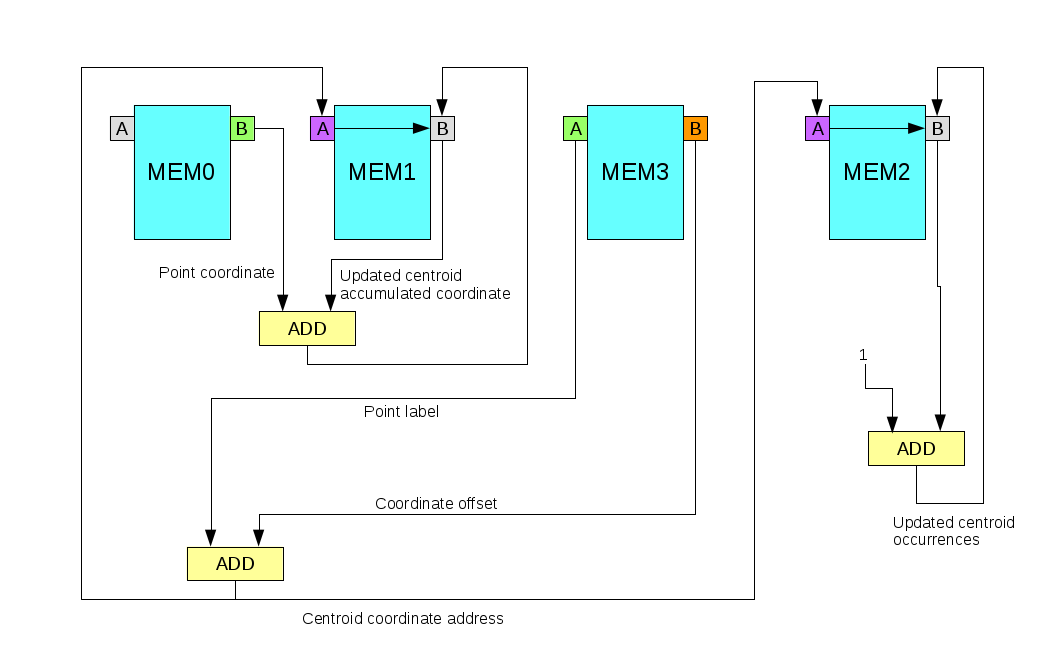
\includegraphics[width=0.85\textwidth]{drawings/kmeans-acc.pdf}
\caption{Datapath for the update step.}
\label{fig:update}
\end{figure}

After the assignment step is done, the datapath for performing the
update step, shown in figure~\ref{fig:update}, is loaded. In this
datapath, the point coordinates, already loaded for the previous step,
are read from port B of MEM0. The point labels (centroid indices),
computed in the previous step, are read from port A of MEM3. Its port
B is generating coordinate offsets synchronized with the datapoint
coordinates. An ALU add labels and coordinate offsets to produce the
accumulated coordinate address of the centroid to update, which is fed
to port A of MEM1. By configuration, port A can serve as the address
for port B, another of Versat's novel features explained in
section~\ref{section:dataEngine}. Thus, the updated centroid
accumulated coordinate is read from port B, added to the current point
coordinate and stored back to port B at the same address. Each port
has an input and an output from which can read an old value and write
a new one to the same address. A similar loop is used for updating the
number of occurrences of each centroid in MEM2, but it only updates
the occurrences once per point. The number of occurrences for each
centroid is stored in MEM2 and is incremented each time it is
addressed, using the same address fed to port A of MEM1. The
incrementer is implemented by another ALU. Note that any FU can select
as input the commonly used constants 0 and 1, instead of a data bus
entry. The two memory read-add-write self loops take 4 clock cycles
due to the accumulated latencies of these operations. Therefore, the
inner loop of the AGUs has size 4 ($Per=4$), and the outer loop size
equals the number of coordinates ($Iter=$ number of coordinates). Also
note that port B of MEM1 and MEM2 are only enabled for writing in the
last cycle of the 4-cycle inner loop ($Duty=1$). After this nested
loop runs, the DE is partially reconfigured to point to the next
datapoint, as is done in the assignment step datapath. This process
repeats until all datapoints in the first chunk are processed.

After the assignment and update steps are run, the next chunk of
datapoints is loaded in MEM0 and the two steps are applied to the new
chunk. This process is repeated until all datapoints are processed.

After all datapoint chunks are processed, the updated centroid
accumulated coordinates reside in MEM1 and must be divided by the
number of occurrences in MEM2 to yield the new centroid
coordinates. Since the DE has no divider, the one that is coupled to
Versat's controller is used to perform the divisions. While the
divider is running, there is time to check whether the newly computed
centroid coordinate differs from the one stored in MEM1, overwriting
it if it does. If none of the new centroids is different from the
stored ones, the algorithm terminates and the final centroids are
DMA transferred to the external memory. If the point labels are also
needed as a final result, then the assignment step must be run again
for all datapoints, as the labels for each data chunk are not
kept. This final loop represents a small overhead if the algorithm has
many iterations. The labels produced during this extra iteration are
DMA transferred to the external memory for each datapoint chunk.

Finally, the program clears register R0 in the CRF, which signals the
host that Versat has finished execution.
 % file "Thesis_Applications.tex"
\cleardoublepage

%\input{Thesis_new_file} % add new .tex files for new chapters
% \cleardoublepage

%\input{Thesis_new_file} % add new .tex files for new chapters
% \cleardoublepage

%%%%%%%%%%%%%%%%%%%%%%%%%%%%%%%%%%%%%%%%%%%%%%%%%%%%%%%%%%%%%%%%%%%%%%%%
%                                                                      %
%     File: Thesis_Results.tex                                         %
%     Tex Master: Thesis.tex                                           %
%                                                                      %
%     Author: Gonçalo Santos                                           %
%     Last modified : 20 Oct 2018                                      %
%                                                                      %
%%%%%%%%%%%%%%%%%%%%%%%%%%%%%%%%%%%%%%%%%%%%%%%%%%%%%%%%%%%%%%%%%%%%%%%%

\chapter{Results}
\label{chapter:results}

The aim of this work is to produce a workable {\bf C} language
compiler for the {\it Versat} architecture using the {\it picoVersat}
instruction set.
The success can be measured by the number of {\bf C} language
constructs that are working properly.
Consequently, testing is of primordial importance, as are the range
of tests used to exercise the compiler.

\section{Functionality}

The compiler, as far the tests were comprehensive,
supports all {\bf C} language integer constructs.
Limitations are listed below.

Since the processor instruction set is reduced, as are the
number of {\bf lcc} terminals to be implemented by the compiler,
the testing of each operation, on its own, is strait
forward.
Testing sequences of such operations may prove more
difficult to test, since different {\bf C} programs
can produce different selection matches.

\section{Testing}

In the test of a compiler, where a small change can affect the
generation of multiple instructions, a good set of
regressive tests is very important.
In order to automate the process, a {\tt test/} directory
was setup.
This directory includes a set of {\bf .c} test files and
the expected output {\bf .out}.

The {\tt Makefile} compiles, executes and compares the new
result with the previously stored result.
All differences in output are printed and can then be analyzed.

Since the output from {\bf iverilog} includes the number
of clocks spent, it is easy to compare whether the changes in the
compiler result in improvements, or in performance degradation.

Some tests are very simple and its output can be easily predicted.
To make testing even simpler, the return value of the {\tt main}
routine is printed, unless the {\sc NORET} environment variables
is defined. Upon return from the {\tt main} routine, the lowest
nibble is printed as an {\sc ASCII} starting at $0$.
This means that values between $10$ and $15$ are printed as
the {\sc ASCII} character at the respective offset, namely the
sequence: \verb|:|, \verb|;|, \verb|<|, \verb|=|, \verb|>|, \verb|?|.

More complex tests can be compiled with {\bf gcc} and executed
to access the expected output.
This, however, can not be performed if the examples include
{\tt asm} calls, since the code can only be executed by the
{\it Versat}, or by the {\bf iverilog} simulator, and not by the
native testbench processor.
%vdb.c

A set of $86$ regression tests is currently being used, ranging
from specific operator testing to complex recursive and iterative
examples. % And the number of tests keeps growing ...

\section{Limitations}\label{limitations}

The {\bf C} language imposes that {\tt sizeof(char)==1}
as does the {\bf lcc} compiler (see~\cite[p.79]{hanson95}).
This works fine as far as {\tt sizeof(char)} can be 32-bits.
However, additionally, the {\bf lcc} assumes through out
the code that $8$ is the number of {\em bit-per-byte}.
If it was a variable, one could set it to $32$.
As it is hardcoded, all address literals
will be truncated to 8-bits ({\tt 8}${}^{\wedge}${\tt ty->size}).
\begin{verbatim}
int *addr = (int*)0x123456;
\end{verbatim}
This can be avoided by setting an integer to the
required value and then assigning it to a pointer.
This works since integer literals are 32-bit wide
and the conversion to pointer, controlled by the
{\it back-end}, does not truncate the value.
\begin{verbatim}
int *addr, value = 0x123456;
addr = (int*)value;
\end{verbatim}
Nevertheless, defining literal pointer is never
a good predictive in virtual memory machines.
In {\it Versat} it is useful to map variables
to specific addresses.

Due to the same reason, a warning message is issued
({\tt shifting an `int' by 12 bits is undefined})
but the code is correctly generated.

% #define LONG_MIN -2147483648
% warning: unsigned operand of unary -
% but 0x80000000 or bellow is OK!
% #  define LONG_MAX	2147483647
% #  define LONG_MIN	(-LONG_MAX - 1L)

In the initial version of {\it picoVersat}, all global
data must be added by {\tt MEM\_BASE=512}.
Since this is performed when addresses are fetched,
static assignments store the unadded value.
Therefore, all accesses must be added by $512$.
Must add {\tt 512} to global pointers in {\tt picoversat-0.0}
\begin{verbatim}
int mem[10], *base = mem;
int main() { base[6+512] = 9; return return mem[6]; }
\end{verbatim}
This can be avoided if assignment is performed during
execution (not at compile time), even if the variable
is global.
\begin{verbatim}
int mem[10];
int main() { int *base = mem; base[6] = 9; return return mem[6]; }
\end{verbatim}

Signed multiplication, division and modulus ({\tt \_mul},
{\tt \_div} and {\tt \_mod}) do not generate carry since
the flags register of {\it picoVersat} is read-only.

The {\bf C} programming languages relies on separate
compilation, where several files are independently
compiled and then linked together.
However, there is no linker in the {\it Versat} system
and the assembler {\bf va} does not support multiple
files.
The solution is to perform linking with {\bf cpp} %%%
include directives.
While in normal {\bf C} the {\tt .c} should be
included, rather compiled, the inclusion of {\bf .h}
as well as {\bf .c} accomplishes the desired result.
Since there is no linking, only multiple inclusion
of files must be avoided.

The {\it Versat} architecture is meant to be used offline
and no form of argument passing to the {\tt main} routine
is available.
Consequently, the stack is initialized at the top.
Therefor, even if the program declares arguments to
the {\tt main} routine ({\tt argc, argv, envp}) they should
never be accessed.
Also, since the system has no memory management unit,
all illegal accesses are silently ignored by the system.
Highly recursive routines that exhaust the stack will have
unpredictable behaviors, since they will begin to overwrite
the top of the code.
Even if it is not the compilers responsibility, it something
that the programmer should be aware, especially when
transitioning from a virtual managed memory system.

Finally, the compiler does not support floating point
data types, since every operation must be supported
by library routines.
This is the case for many android devices, namely
smartphones.
However, the {\it Versat} purpose is to perform
integer arithmetic operations fast and is not aimed at
scientific programming.
The error message {\tt compiler error in \_label--Bad terminal}
is issued by the compiler when it cannot handle a given operation,
namely floating point operations.

\section{Register assignment}

Register assignment in compiler design considers two types of registers:
global registers that hold variable values and scratch registers that hold
temporary values.
The {\bf lcc} compiler defines these registers by setting a mask for each
type of register.
It is up to each {\it back-end} to define the mask values according to processor
capabilities.
For instance, the {\bf sparc} processor defines $4$ sets of $8$ registers:
global, temporary, input and output; where the later two sets replace
the stack for argument passing.
In {\bf i386} all $7$ registers are temporary, while {\bf mips} uses half
for each purpose ($16+16$).

Since the {\it picoVersat} has no specific register assignment, a study
was carried out in order to assess the best balance between global and
scratch registers.
Registers {\tt R0} and {\tt R13} to {\tt R15} are used to communicate with {\it Versat}
and are invisible to the compiler.
The stack is controlled by a {\it stack pointer} ({\tt R12}) and a {\it frame pointer}
({\tt R11}).
The remaining registers ({\tt R1} to {\tt R10}) compose a mask {\tt 7FE}, where
the lowest bit ({\tt R0}) is omitted for register assignment, and the highest
used bit {\tt 400} is {\tt R10}.
The register {\tt R1} is used to return function values and all arguments are
passed on the stack.
At least two registers must be used as scratch for binary operations
temporaries.
The compiler allows the definition of a {\tt tmask} for temporaries and a
{\tt vmask} for variables.

Initially, in run $1$, the experiment uses all registers for temporaries.
Each run adds a variable register at the expense of a temporary, until only
two temporaries remain (run $9$).
Three examples where used: {\tt assign}, {\tt repeating locals} and
{\tt bubble sort}.
The first two represent opposite extremes of register usage, while the last is
a more balanced and realistic example.

The first example uses the {\bf C} language right associative {\it assign} operator
where each new assignment to the variable {\tt a} requires a new temporary register.
%(see Figure~\ref{fig:assign}).

%\begin{figure}
\begin{verbatim}
int f() { return 1; }
int main()
{
  int a;

  a = f() + (a =
      f() + (a =
      f() + (a =
      f() + (a =
      f() + (a =
      f() + (a =
      f() + (a =
      f() + (a =
      f() + (a =
      f() + (a =
      f() + (a =
      f() + (a =
      f() + (a = 1
                  )))))))))))));
  return a;
}
\end{verbatim}
%\caption{}
%\end{figure}

The register usage shows that each assign uses a register $4$ times at
the expense of the return register {\tt R1}.
The best solution, represented by the lowest clock count,
is to use only two temporaries, since more variables imply more stack ({\tt R12}),
saves and restores between each call to the function {\bf f}.

%\begin{table}
\begin{center}
{\small
\begin{tabular}{r|r|r|r|r|r|r|r|r|r|r|r|r|r|r|r|r}
run&vars&vmask&tmask&R1&R2&R3&R4&R5&R6&R7&R8&R9&R10&R11&R12&clks\\\hline
1&0&000&7FE&21&4&4&4&4&4&4&4&6&44&27&82&677\\
2&1&400&3FE&23&4&4&4&4&4&4&6&42&17&14&82&638\\
3&2&600&1FE&25&4&4&4&4&4&6&42&0&17&16&77&633\\
4&3&700&0FE&27&4&4&4&4&6&42&0&0&17&18&72&628\\
5&4&780&07E&29&4&4&4&6&42&0&0&0&17&20&67&623\\
6&5&7C0&03E&31&4&4&6&42&0&0&0&0&17&22&62&618\\
7&6&7E0&01E&33&4&6&42&0&0&0&0&0&17&24&57&613\\
8&7&7F0&00E&35&6&42&0&0&0&0&0&0&17&26&52&608\\
9&8&7F8&006&39&42&0&0&0&0&0&0&0&17&28&47&603\\
\end{tabular}
}
\end{center}
%\caption{}
%\end{table}
\vspace*{5mm}

The second example uses lots of repeating local variables so that each one is assigned
a register, for its uses from the first to last line, if one is available.
%(see Figure~\ref{fig:locals}).

%\begin{figure}
\begin{verbatim}
int func(int a, int b, int c, int d, int e, int f, int g, int h, int i, int j, int k) {
    a = a + b - c - d - e + f - g + h + i + j + k;
    b = a - b + c + d - e - f + g - h + i - j - k;
    c = a + b - c - d + e + f + g - h + i + j - k;
    d = a - b - c + d - e + f - g + h - i - j - k;
    e = a + b + c - d - e - f - g + h - i + j - k;
    f = a - b - c + d - e + f + g - h - i - j + k;
    g = a + b - c - d + e + f + g - h + i + j - k;
    h = a - b + c + d - e - f - g + h + i - j - k;
    i = a + b - c - d - e + f + g + h + i + j - k;
    j = a - b - c + d - e + f + g - h - i - j - k;
    k = a + b + c - d + e - f - g - h - i + j + k;
    return a + b + c + d + e + f - g + h - i + j - k;
}

int main() {
    return func(10, 9, 8, 7, 6, 5, 4, 3, 2, 1, 0);
}
\end{verbatim}
%\caption{}
%\end{figure}

As expected, the best solution is to use highest of temporaries in order
to reduce frame pointer ({\tt R11}) accesses to stack saved values.

%\begin{table}
\begin{center}
{\small
\begin{tabular}{r|r|r|r|r|r|r|r|r|r|r|r|r|r|r|r|r}
run&vars&vmask&tmask&R1&R2&R3&R4&R5&R6&R7&R8&R9&R10&R11&R12&clks\\\hline
1&0&000&7FE&45&27&12&13&48&46&40&45&54&62&68&56&956\\
2&1&400&3FE&53&31&13&54&46&40&47&54&62&0&78&51&1001\\
3&2&600&1FE&61&35&52&46&48&49&56&62&0&0&89&46&1051\\
4&3&700&0FE&89&39&59&63&51&56&62&0&0&0&101&41&1106\\
5&4&780&07E&109&43&75&49&74&79&0&0&0&0&113&36&1161\\
6&5&7C0&03E&146&45&84&58&105&0&0&0&0&0&124&31&1211\\
7&6&7E0&01E&156&88&112&94&0&0&0&0&0&0&138&26&1278\\
8&7&7F0&00E&171&117&176&0&0&0&0&0&0&0&154&21&1356\\
9&8&7F8&006&231&249&0&0&0&0&0&0&0&0&172&16&1447\\
\end{tabular}
}
\end{center}
%\caption{}
%\end{table}
\vspace*{5mm}

The last example, the {\it bubble sort}, uses a mixture temporaries and variable
reuses. %(see Figure~\ref{fig:bubble}).

%\begin{figure}
\begin{verbatim}
#include "printi.h"

int bubble(int list[], int n) {
    int c, d, t, swap, cnt = 0;

    for (c = 0; c < n - 1; c++) {
        for (swap = 0, d = n - 1; d > c; d--)
            if (list[d - 1] > list[d]) {    /* Swapping */
                swap++;
                t = list[d];
                list[d] = list[d - 1];
                list[d - 1] = t;
            }
        if (!swap)
            break;
        cnt++;
    }
    return cnt;
}

int v[] = { 7, 4, 9, 6, 2, 1, 3, 5, 8, 0 };

int main() {
    int i, size = sizeof(v) / sizeof(v[0]), cnt = bubble(v, size);
    for (i = 0; i < size; i++) {
        putchar(v[i] + '0');
        putchar(' ');
    }
    printi(cnt, 10);
    putchar('\n');
    return 0;
}
\end{verbatim}
%\caption{}
%\end{figure}

This example exploits the tradeoff between global and temporary register
usage.
In the first runs the compiler is unable to use all temporaries.
In the last runs some variable registers are left unassigned and the number
of required execution clocks rises again.

%\begin{table}
\begin{center}
{\small
\begin{tabular}{r|r|r|r|r|r|r|r|r|r|r|r|r|r|r|r|r}
run&vars&vmask&tmask&R1&R2&R3&R4&R5&R6&R7&R8&R9&R10&R11&R12&clks\\\hline
1&0&000&7FE&2&0&0&0&0&4&5&15&30&45&31&36&9855\\
2&1&400&3FE&2&0&0&0&0&4&7&29&41&11&24&36&8193\\
3&2&600&1FE&2&0&0&0&4&5&27&37&7&11&19&41&7714\\
4&3&700&0FE&2&0&0&0&5&25&37&4&7&11&17&41&7399\\
5&4&780&07E&2&0&0&5&19&37&6&4&7&11&13&46&7022\\
6&5&7C0&03E&2&0&5&19&33&6&6&4&7&11&9&49&6949\\
7&6&7E0&01E&2&5&19&33&0&6&6&4&7&11&9&49&6949\\
8&7&7F0&00E&5&19&33&0&0&6&6&4&7&11&9&44&6921\\
9&8&7F8&006&21&28&0&0&0&6&6&4&7&11&13&41&7492\\
\end{tabular}
}
\end{center}
%\caption{}
%\end{table}
\vspace*{5mm}

Based on experience with the examples above, a balanced approach should work best
in most cases.
Therefor, the first five registers, {\tt R1} to {\tt R5}, are used as temporaries
({\tt tmask=0x003E}) and the remaining five, {\tt R6} to {\tt R10}, are used as
variables ({\tt vmask=0x07C0}).

\section{Efficiency considerations}

Calls are very expensive operations for any processor.
{\it Intel Inc.} has made a significant effort over the year to address this
problem.
In the last years, its high end processors provide faster {\it calls} than
{\it jumps} at the expense of higher transistor count. %ref!
In a processor like {\it picoVersat}, the problem is magnified since
no stack specific registers or opcodes are available.

A function call in the {\bf C} programming language requires:
\begin{enumerate} \itemsep0em 
\item {\bf argument passing} by pushing values to the stack;
\item {\bf calling} the desired routine;
\item {\bf saving used registers} before the routine destroys its values;
\item {\bf frame pointer} saving to access arguments and locals;
\item {\bf allocate space} for local variables;
\item actually performing the routine operations;
\item {\bf restoring frame pointer} of the previous routine;
\item {\bf restoring used registers} previous values;
\item {\bf returning} to the calling routine;
\item {\bf removing arguments} from stack.
\end{enumerate}
The present compiler detects when a routine accesses no arguments or locals
and does not emit frame pointer code. So, if a routine only uses global
variables, the call becomes a bit more efficient.
Some of the tests used become upto 5\% faster by removing the frame
pointer in routines where it not needed.

As any routine can be called many times, even recursively, the compiler
must save, at the beginning, and restore, at the end,
all the registers the routine uses.
This means that, at the start of the program, the {\tt main} routine will spill
all registers it will use, although they have no defined value.
Such procedure is required since the routine may be recursively called.
However, in most cases, the {\tt main} routine is only invoked once, at
the start of the program.
The {\sc NOSAV} environment variable can be set if the {\tt main}
routine is not used recursively and no registers will saved by the compiler.
This special hack can be dangerous to use, but it makes {\tt main} based
programs more efficient.

The {\it picoVersat} controls {\it Versat} by setting specific values to
predefined memory positions.
The use of a routine to perform such a task is a very
expensive way to change memory positions, either through {\tt asm}
directives or standard {\bf C} code, as the tests {\tt set.c} and
{\tt setvar.c} show, respectively.
Memory values can be efficiently changed by assigning to a pointer
{\tt *addr=val} (see Limitations, above).

During this work, the {\it picoVersat} evolved. The use of a single
memory, for program code and data, removed the need for a {\tt addi MEM\_BASE}
instruction for each variable load and store, resulting in a 5\% improvement
over all the regression test in use, at the time. % 17022/16213 pico-0

Finally, the compiler some times generates a register read after the
same register was written by another instruction selection.
At least, the read can be suppressed, but {\bf lcc} provides no
peephole optimizer for final code cleanup.

\section{Compiler instalation}

The compiler itself, {\bf lcc}, can be invoqued directly with the
{\tt -target=versat} option, as long as the input file has already
been preprocessed ({\bf cpp}).
The compiler output is a {\it picoVersat} assembly, that can then
fed to the {\it versat} assembler ({\bf va}).

However, the complete compilation process, from {\bf C} language
source file to {\bf iverilog} simulation executable, can be
integrated as in a standard high-level compiler.

Section~\ref{app:integ} describes the requirements for such an integration.
The compiler {\tt Makefile}s, in the main and {\tt versat/} directories,
can be used to provide the instalation of all required files
for a complete development environment.
By default, without any changes to the {\tt Makefile}s, the
compiler development environment is placed under the
{\tt /usr/local/versat} directory.

The default directories for the compiler installation
({\tt make install}) are predefined as
{\tt /usr/local/versat/lcc} for the compiler files
({\tt lcc}, {\tt cpp}, {\tt rcc}, {\tt va}, and
{\tt xdict.json}), and can be redefined at compile
time or using the {\sc LCCDIR} environment variable
at runtime. The {\it picoVersat} {\tt rtl/} files
({\tt include/}, {\tt src/}, and {\tt testbench/})
should be copied to {\tt /usr/local/versat/pico}
(defined at compile time).
Also the {\bf iverilog} compiler is defined at
compile time as residing in {\tt /usr/local/bin/}.

The structure of the installed files,
in the current version is:
\begin{Verbatim}[baselinestretch=1.0]
/usr/local/versat/lcc/lcc
/usr/local/versat/lcc/cpp
/usr/local/versat/lcc/rcc
/usr/local/versat/lcc/va
/usr/local/versat/lcc/xdict.json
/usr/local/versat/lcc/include/strlen.h
/usr/local/versat/lcc/include/umod.h
/usr/local/versat/lcc/include/errno.h
/usr/local/versat/lcc/include/malloc.h
/usr/local/versat/lcc/include/umul.h
/usr/local/versat/lcc/include/itoa.h
/usr/local/versat/lcc/include/Makefile
/usr/local/versat/lcc/include/stdarg.h
/usr/local/versat/lcc/include/mem_ends.h
/usr/local/versat/lcc/include/xdict.h
/usr/local/versat/lcc/include/atoi.h
/usr/local/versat/lcc/include/puts.h
/usr/local/versat/lcc/include/dma.h
/usr/local/versat/lcc/include/versat.h
/usr/local/versat/lcc/include/ends.h
/usr/local/versat/lcc/include/mul.h
/usr/local/versat/lcc/include/xdictinc
/usr/local/versat/lcc/include/div.h
/usr/local/versat/lcc/include/ends.cbc
/usr/local/versat/lcc/include/udiv.h
/usr/local/versat/lcc/include/printf.h
/usr/local/versat/lcc/include/mod.h
/usr/local/versat/lcc/include/alloca.h
/usr/local/versat/lcc/include/printi.h
/usr/local/versat/lcc/include/gnuc.h
/usr/local/versat/lcc/include/putchar.h
/usr/local/versat/lcc/include/assign.h
/usr/local/versat/pico/testbench/sim_xtop.cpp
/usr/local/versat/pico/testbench/xtop_tb.v
/usr/local/versat/pico/include/xdefs.vh
/usr/local/versat/pico/src/xaddr_decoder.v
/usr/local/versat/pico/src/xctrl.v
/usr/local/versat/pico/src/xram.v
/usr/local/versat/pico/src/xregf.v
/usr/local/versat/pico/src/xcprint.v
/usr/local/versat/pico/src/xtop.v
\end{Verbatim}

After adding the {\tt /usr/local/versat/lcc} directory to
the {\sc PATH} environment variable, an executable example
can be produced with the command:\\
{\tt lcc example.c -o example}

The example can then be run with:\\
{\tt ./example}

Please note that the {\it versat} memory dump {\tt .hex}
file is stored in the {\tt /tmp} directory.

\cleardoublepage
 % file "Thesis_Results.tex"
\cleardoublepage

%%%%%%%%%%%%%%%%%%%%%%%%%%%%%%%%%%%%%%%%%%%%%%%%%%%%%%%%%%%%%%%%%%%%%%%%
%                                                                      %
%     File: Thesis_Conclusions.tex                                     %
%     Tex Master: Thesis.tex                                           %
%                                                                      %
%     Author: Carlos A. Rodrigues                                      %
%     Last modified : 21 Jan 2011                                      %
%                                                                      %
%%%%%%%%%%%%%%%%%%%%%%%%%%%%%%%%%%%%%%%%%%%%%%%%%%%%%%%%%%%%%%%%%%%%%%%%

\chapter{Conclusão}
\label{chapter:conclusao}

Insert your chapter material here...


% ----------------------------------------------------------------------
\section{Achievements}
\label{section:achievements}

The major achievements of the present work...


% ----------------------------------------------------------------------
\section{Trabalho Futuro}
\label{section:futuro}

dese


\cleardoublepage

 % file "Thesis_Conclusions.tex"
\cleardoublepage

% ----------------------------------------------------------------------
%  Bibliography
% ----------------------------------------------------------------------

% Add entry in the table of contents as chapter
\phantomsection
\addcontentsline{toc}{chapter}{\bibname}

% Include all references in .bib file, even non-cited ones...
%\nocite{*} % this should be used carefully because it is not correct!

% Produces the bibliography section when processed by BibTeX
%
% Bibliography style
% > entries ordered alphabetically
%\bibliographystyle{plain}
% > unsorted with entries appearing in the order in which the citations appear.
%\bibliographystyle{unsrt}
% > entries ordered alphabetically, with first names and names of journals and months abbreviated
%\bibliographystyle{abbrv}
% > entries ordered alphabetically, with reference markers based on authors' initials and publication year
%\bibliographystyle{alpha}
%
% Replacement bibliography styles provided by 'natbib' package
% (plainnat.bst, abbrvnat.bst, unsrtnat.bst )
% > entries ordered alphabetically
%\bibliographystyle{plainnat}
% > unsorted with entries appearing in the order in which the citations appear.
%\bibliographystyle{unsrtnat}
% > entries ordered alphabetically, with first names and names of journals and months abbreviated
%\bibliographystyle{abbrvnat} % <<<<< SELECT IF USING REFERENCES BY AUTHOR/YEAR
% > entries ordered alphabetically, with reference markers based on authors' initials and publication year
%\bibliographystyle{alpha}
%
% Custom bibliography style adapted from 'natbib' package
%   (based on http://tex.stackexchange.com/questions/5053/is-it-possible-to-get-unsrt-abbrv-bibliography)
%   (unsrtnat.bst + abbrvnat.bst -> abbrvunsrtnat.bst)
%   (original files copied from:
%   http://tug.ctan.org/macros/latex/contrib/natbib/abbrvnat.bst
%   http://tug.ctan.org/macros/latex/contrib/natbib/unsrtnat.bst
% > unsorted with entries appearing in the order in which the citations appear, with first names and names of journals and months abbreviated.
\bibliographystyle{abbrvunsrtnat} % <<<<< SELECT IF USING REFERENCES BY NUMBER (CITATION ORDER)

% External bibliography database file in the BibTeX format
\bibliography{Thesis_bib_DB} % file "Thesis_bib_DB.bib"

%\cleardoublepage

% ----------------------------------------------------------------------
%  Appendix (optional)
%
%  CAUTION: 1) the main document (up to the conclusions) shall not exceed 80 pages
%           2) the document shall not exceed a total of 100 pages (per IST regulations)
% ----------------------------------------------------------------------
\appendix

% add page number prefix according to apendix chapter (optional)
%\renewcommand{\thepage}{\thechapter.\arabic{page}}

% re-set arabic numbering (A.1,A.2,...) (optional, use only if chapter prefix is added)
%\setcounter{page}{1}

%%%%%%%%%%%%%%%%%%%%%%%%%%%%%%%%%%%%%%%%%%%%%%%%%%%%%%%%%%%%%%%%%%%%%%%%%
%                                                                      %
%     File: Thesis_Appendix_A.tex                                      %
%     Tex Master: Thesis.tex                                           %
%                                                                      %
%     Author: Andre C. Marta                                           %
%     Last modified :  2 Jul 2015                                      %
%                                                                      %
%%%%%%%%%%%%%%%%%%%%%%%%%%%%%%%%%%%%%%%%%%%%%%%%%%%%%%%%%%%%%%%%%%%%%%%%

\chapter{Vector calculus}
\label{chapter:appendixVectors}

In case an appendix if deemed necessary, the document cannot exceed a total of 100 pages...

Some definitions and vector identities are listed in the section below.

% ----------------------------------------------------------------------
\section{Vector identities}
\label{section:vectorIdentities}

\begin{equation}
	\nabla \times \left( \nabla \phi \right) = 0
	\label{eq:cross_nnp}
\end{equation}

\begin{equation}
	\nabla \cdot \left( \nabla \times {\bf u} \right) = 0
	\label{eq:dotCross_nnu}
\end{equation}

 % file "Thesis_Appendix_A.tex"
%\cleardoublepage

% re-set arabic numbering (B.1,B.2,...) (optional, use only if chapter prefix is added)
%\setcounter{page}{1}

%%%%%%%%%%%%%%%%%%%%%%%%%%%%%%%%%%%%%%%%%%%%%%%%%%%%%%%%%%%%%%%%%%%%%%%%%
%                                                                      %
%     File: Thesis_Appendix_B.tex                                      %
%     Tex Master: Thesis.tex                                           %
%                                                                      %
%     Author: Andre C. Marta                                           %
%     Last modified :  2 Jul 2015                                      %
%                                                                      %
%%%%%%%%%%%%%%%%%%%%%%%%%%%%%%%%%%%%%%%%%%%%%%%%%%%%%%%%%%%%%%%%%%%%%%%%

\chapter{Technical Datasheets}
\label{chapter:appendixDatasheets}

It is possible to add PDF files to the document, such as technical sheets of some equipment used in the work.

% ----------------------------------------------------------------------
\section{Some Datasheet}
\label{section:datasheet}

% See more options to include PDF files in
% http://mirror.unl.edu/ctan/macros/latex/contrib/pdfpages/pdfpages.pdf
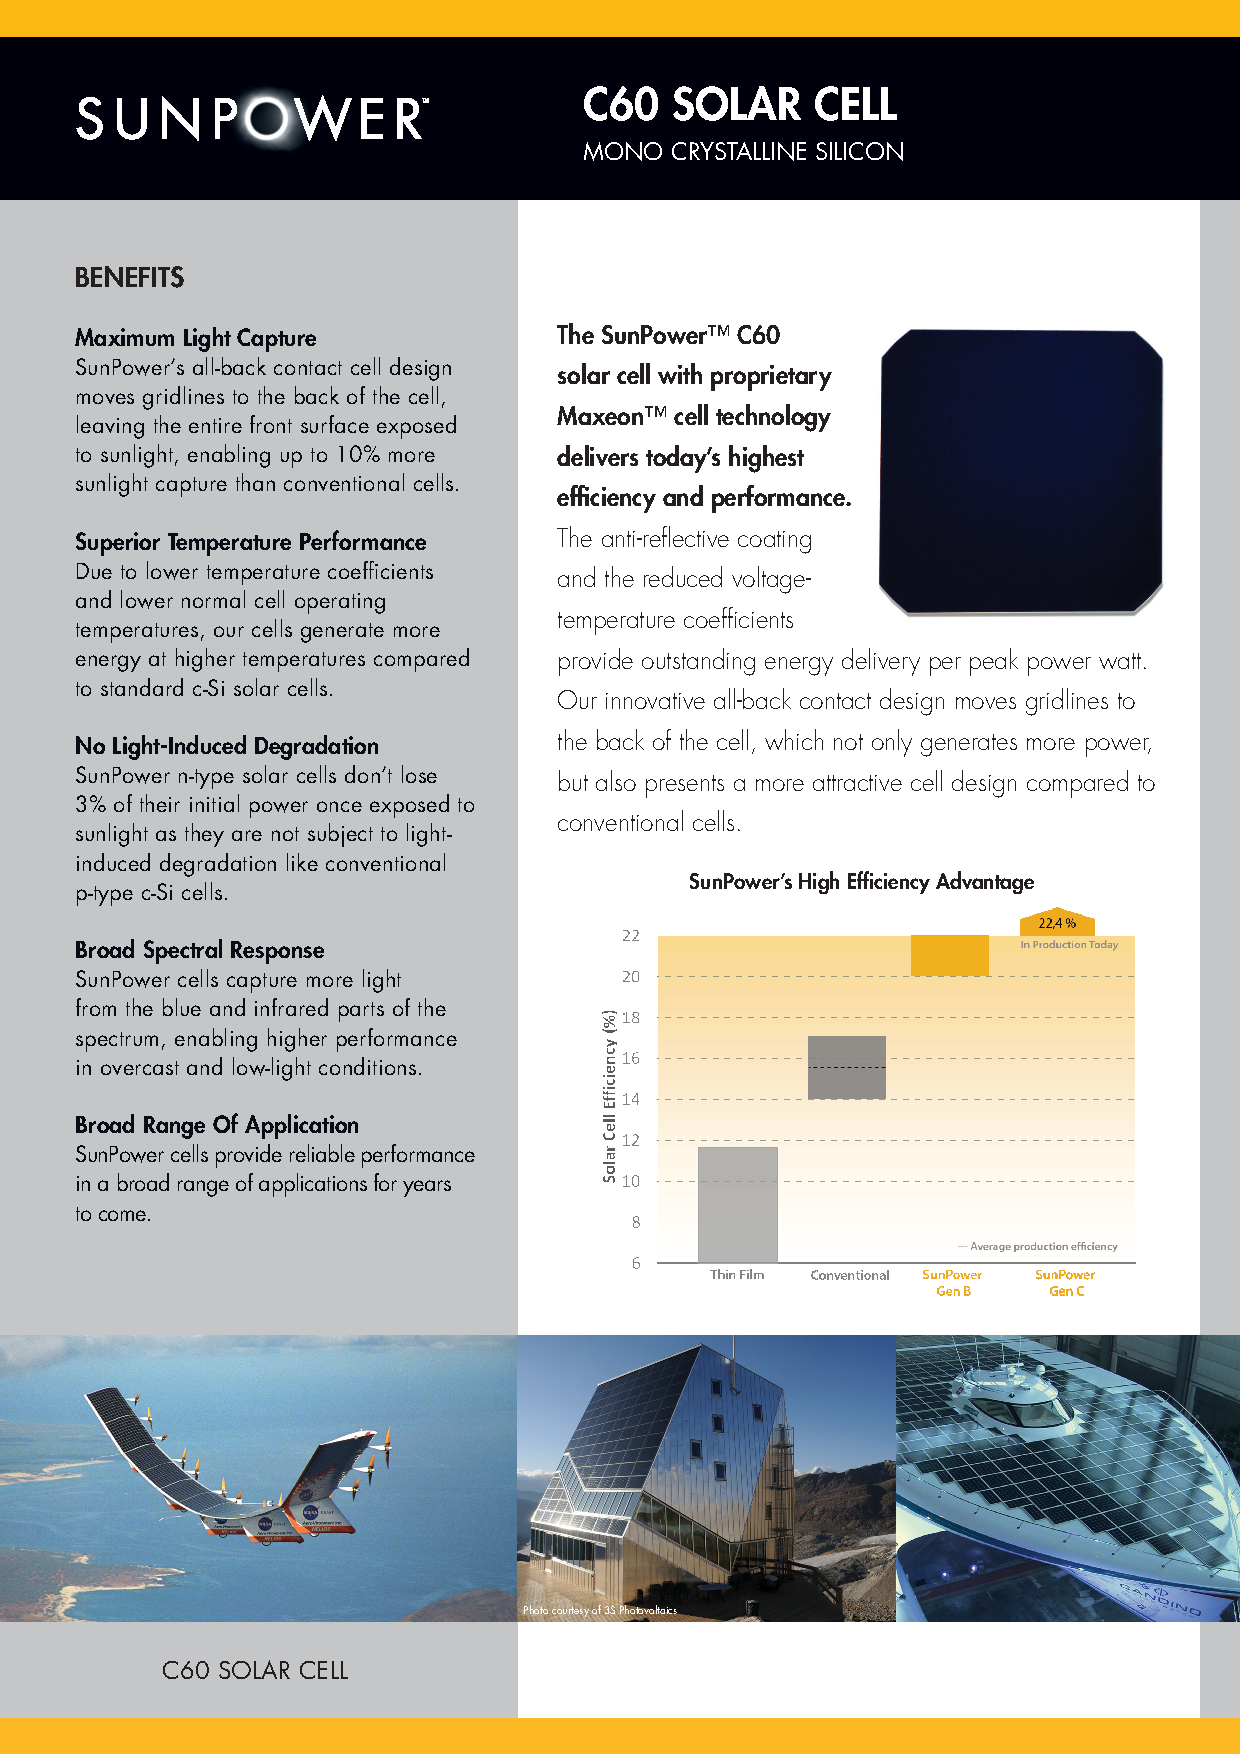
\includepdf[pages={1-2},nup=1x2,landscape=true]{Figures/SolarCell_Sunpower_C60.pdf}

 % file "Thesis_Appendix_B.tex"
%\cleardoublepage

% ----------------------------------------------------------------------
\end{document}
% ----------------------------------------------------------------------

